
\begin{abstract}
  This report present the work carried out during my Master's Thesis in the Megason Lab, Harvard Medical School, Boston MA, USA.
  This internship is the last step of my formation in the National Institute of Applied Sciences of Lyon (INSA), and at the University Claude Bernard Lyon 1 (UCLB), to get the Master of Sciences in Electrical engineering and Proceeds, option Systems and Images, and the Master of Engineering in Electrical Engineering and Computer Sciences.

  The work presented here is based on microscopy images processing. I have been working on three dimension plus time datasets representing a developing zebra fish embryo. 
  The laboratory employs a team of computer scientists in charge of development of a program for biological data visualization and processing :{\gofigure}\cite{refGofigure2}.
  The project carried out while in the Megason Lab intend to be integrated to this program.
  
\tableofcontents  
  
 
\end{abstract}


\chapter{Context}

\begin{figure}[htb]
\begin{center}
\leavevmode
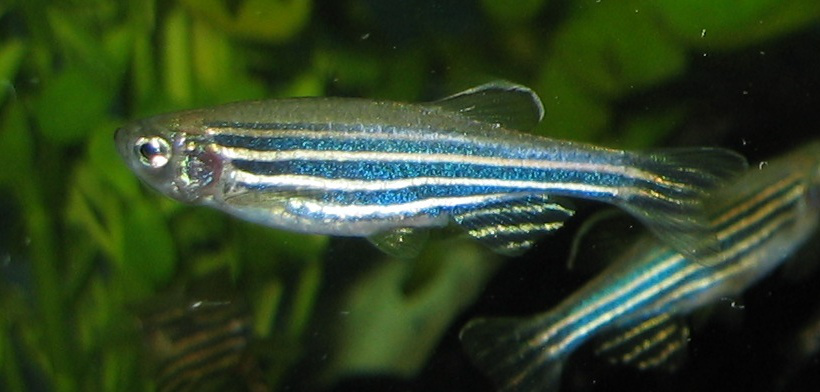
\includegraphics[width=0.99\textwidth]{pictures/zebrafishPic}
\end{center}
\caption{Mature zebra fish: approximatively 2.5cm long (source: \href{http://en.wikipedia.org/wiki/File:Zebrafisch.jpg}{Wikipedia})}
\label{fig:ZebraPic}
\end{figure}

\section{Systems Biology}

With the completion of the genome projects~\cite{}, the stage is now set for a
more complete understanding of how animals are created. Biologists now have
access to the complete sequence of DNA that encodes the blueprint of life for
many animals including human, mouse, zebrafish, and fruit
fly~\cite{[2][3][4][5]} \TODO{refe?}The challenge is now understanding how this
code functions. The problem however is that the only thing that biologists can
currently reliably predict from the genomic code is which parts can be
transcribed and translated into protein. Biologists cannot accurately predict
when and where a protein will be expressed, how a protein will
function once it is created, and the interaction between expressed proteins that
allow them to form functional genetic circuits. Thus, although the genome
projects have given us the complete code for constructing many organisms, the
only part of the code biologists can currently read is the parts list. The
challenge is understanding how all these parts fit together to form molecular
circuits, how these circuits process information to regulate the behavior of
cells, and how the behavior of cells is orchestrated to generate functional form
as in \emph{embryogenesis}. This post-genomic endeavor has come to be called
\emph{systems biology}.\\

Although systems biology grew out of the “-omics” field which made heavy use of 
in vitro biochemical approaches (e.g. sequencing, microarrays, and proteomics),
\textit{in-vivo} imaging is becoming an increasingly powerful tool for
systems biology. \textit{In-vivo} imaging is advantageous over
biochemical approaches for doing systems biology:

\begin{itemize}
 \item Biological circuits function at the single cell level. Microscopic
imaging easily achieves this resolution while in-vitro techniques do not.
 \item Biological circuits function over time. With imaging, different
components of a biological circuit can be labeled using different colors of
fluorescent proteins and the dynamics of the circuit monitored non-invasively
with time-lapse fluorescent imaging as the circuit functions in an intact
system. In vitro biochemical approaches typically require the tissue to
be destroyed in order to be assayed which precludes longitudinal analysis.
 \item the quantitative amounts of components in a biological circuit are
important for its function. Fluorescent imaging can accurately quantitate the
levels of molecular components even at the protein level through the use of
fluorescent protein (e.g. GFP) fusions. Omic approaches are typically less
quantitative and focus at the DNA or RNA level which is less relevant.
 \item the anatomical context of biological circuits is essential for
determining their function; the use of spatial cues to generate different cell
types in different places is a fundamental aspect of development. In vivo
imaging can capture data from intact animals preserving its anatomical context.
In vitro approaches typically grind up the tissue to assay it, thus destroying
its anatomy.
\end{itemize}

%%%%%%%%%%%%%%%%%%%%%%%%%%%%%%%%%%%%%%%%%%%%%%%%%%%%%%%%%%%%%%%%%%%%%%%%%%%%%%%
%%%%%%%%%%%%%%%%%%%%%%%%%%%%%%%%%%%%%%%%%%%%%%%%%%%%%%%%%%%%%%%%%%%%%%%%%%%%%%%
%%%%%%%%%%%%%%%%%%%%%%%%%%%%%%%%%%%%%%%%%%%%%%%%%%%%%%%%%%%%%%%%%%%%%%%%%%%%%%%

\section{Zebrafish: one sytem of high interest for Systems-Biology}

Zebrafish (Danio rerio) is a small, freshwater, tropical fish commonly available
in pet stores (see figure~\ref{}). It has become a popular model system for the
study of genetics and development in the last 2 decades and there are now
many labs worldwide that study it. There have been several
large-scale mutagenesis screens caried out in zebrafish and its genome has been
largely sequenced. Zebrafish has the advantages of fruit fly in that it
is amenable to forward genetic screens, but unlike fruit fly, zebrafish is a
vertebrate so is much more relevant to humans. Another huge advantage
of zebrafish is its suitability for imaging. Zebrafish embryos are transparent,
small, develop freely outside their mother, and develop directly from egg to
adult without any larval stages. This means that a zebrafish egg can be placed
under a microscope and continuously imaged throughout embryogenesis. This would
be impossible with a mouse which develop inside its mother, with a frog
(Xenopus) egg which is opaque, or with a fruit fly (Drosophila) which has
several larval/pupal stages and is opaque.

%%%%%%%%%%%%%%%%%%%%%%%%%%%%%%%%%%%%%%%%%%%%%%%%%%%%%%%%%%%%%%%%%%%%%%%%%%%%%%%
%%%%%%%%%%%%%%%%%%%%%%%%%%%%%%%%%%%%%%%%%%%%%%%%%%%%%%%%%%%%%%%%%%%%%%%%%%%%%%%
%%%%%%%%%%%%%%%%%%%%%%%%%%%%%%%%%%%%%%%%%%%%%%%%%%%%%%%%%%%%%%%%%%%%%%%%%%%%%%%

\section{In-toto imaging: one technique of interest for Systems-Biology}

The goal of in toto imaging is to image and track every single cell in a
developing tissue, organ, or eventually
whole embryo~\cite{megason2003digitizing}. This technique will provide
significant outcomes in a complete understanding of the cellular basis of
development through the construction of complete lineage trees\footnote{First
results on early zebrafish embryo~\cite{SCIENCE-PAPER} show the immense impact
on the scientific community of such a technique.}. There are several steps to in
toto imaging.\\

The embryos must first be labeled with “segmentation markers” which allow all
the cells to be segmented. Additionally embryos can be labeled with additional
markers to reveal RNA or protein expression. The next step is to acquire 3D+t
image sets using confocal or 2-photon fluorescent microscopy. And the final step
is processing the often very large image sets to segment out all the cell
trajectories and to extract quantitative, cell-centric data.

\subsection{Embryo Labeling}

The living embryos must be labeled with fluorescent markers and imaged with
time-lapse technique. Biologists must use vital labels such as Green
Fluorescent Protein (GFP), or other available Fluorescence Proteins (FPs) across
the visible spectrum. Since FPs are proteins rather than organically synthesized
small molecule dyes, FPs can be endogenously expressed by transgenic organisms
and are open to all the power of genetic engineering.\\

There are 2 basic uses of markers for in toto imaging: segmentation and
expression.
\begin{itemize}
 \item Segmentation markers allow the cells to be segmented in space,
across time, and across cell-division. Biologists, at the Megason Lab, typically
use a histone-FP of one color (e.g. histone-cerulean) and a membrane-localized
FP of another color (e.g. membrane-mCherry). This combination would generate
embryos in which every nuclei is green and all the cell membranes are red~(see
figure~\ref{}).
 \item Expression markers refer to whatever else is being marked such that it
can be digitized with in toto imaging. For example, transgenic fish can be made
that express a fluorescent protein wherever some gene is normally expressed
during development.
\end{itemize}

%%%%%%%%%%%%%%%%%%%%%%%%%%%%%%%%%%%%%%%%%%%%%%%%%%%%%%%%%%%%%%%%%%%%%%%%%%%%%%%
%%%%%%%%%%%%%%%%%%%%%%%%%%%%%%%%%%%%%%%%%%%%%%%%%%%%%%%%%%%%%%%%%%%%%%%%%%%%%%%
%%%%%%%%%%%%%%%%%%%%%%%%%%%%%%%%%%%%%%%%%%%%%%%%%%%%%%%%%%%%%%%%%%%%%%%%%%%%%%%

\subsection{Image acquisition}

\subsubsection{Requirements}

In toto imaging tracks cells during development only by the correspondence of
cells from frame to frame. This is quite different than traditional fate mapping
in developmental biology where only a small subset of cells is labeled at one
stage of development and the location of their progeny is observed at a
later stage. In toto imaging thus requires images that have high enough
resolution in space to resolve all the cells (this requires $\approx
1 \mu$m resolution) and high enough resolution in time to not lose track of
moving and dividing cells (this requires $\approx 2$ min time resolution). In
addition to high resolution, in toto imaging also requires complete coverage.
All the cells of interest must be continuously imaged in order to be tracked; if
cells leave the field of view then their lineage cannot be completely tracked.

\subsubsection{Equipment}

Achieving both high spatial and temporal resolution as well as complete coverage
can be achieved through the use of time-lapse confocal or 2-photon microscopy.
Confocal microscopy~(see figure~\ref{fig:ConfocalPrinciple}) uses a pinhole to
eliminate out of focus light whereas 2-photon microscopy only excites
fluorescence in the focal plane.

Thus both techniques allow thin (1$\mu$m) optical sections of fluorescent
samples to be captured. By imaging at a series of focal planes, stacks of
optical sections can be captured to generate a volumetric image and this can be
repeated over time to generate 3D+t images. The axial (z) resolution with these
techniques is typically around 5-fold less than the planar (xy) resolution so
the volumetric images are anisotropic. Confocal imaging provides 2-fold higer
resolution than 2-photon imaging but has a depth penetration limit of  150 um.
2-photon imaging can image all the way through a zebrafish embryo and has
reduced phototoxicity to the embryo and photobleaching of the fluorescent
labels.\\

Both acquisition techniques have been assembled in the Megasaon Lab from a
Zeiss 710 NLO (figure~\ref{fig:MicMegason}).


\begin{figure}[htb]
\begin{center}
\leavevmode
 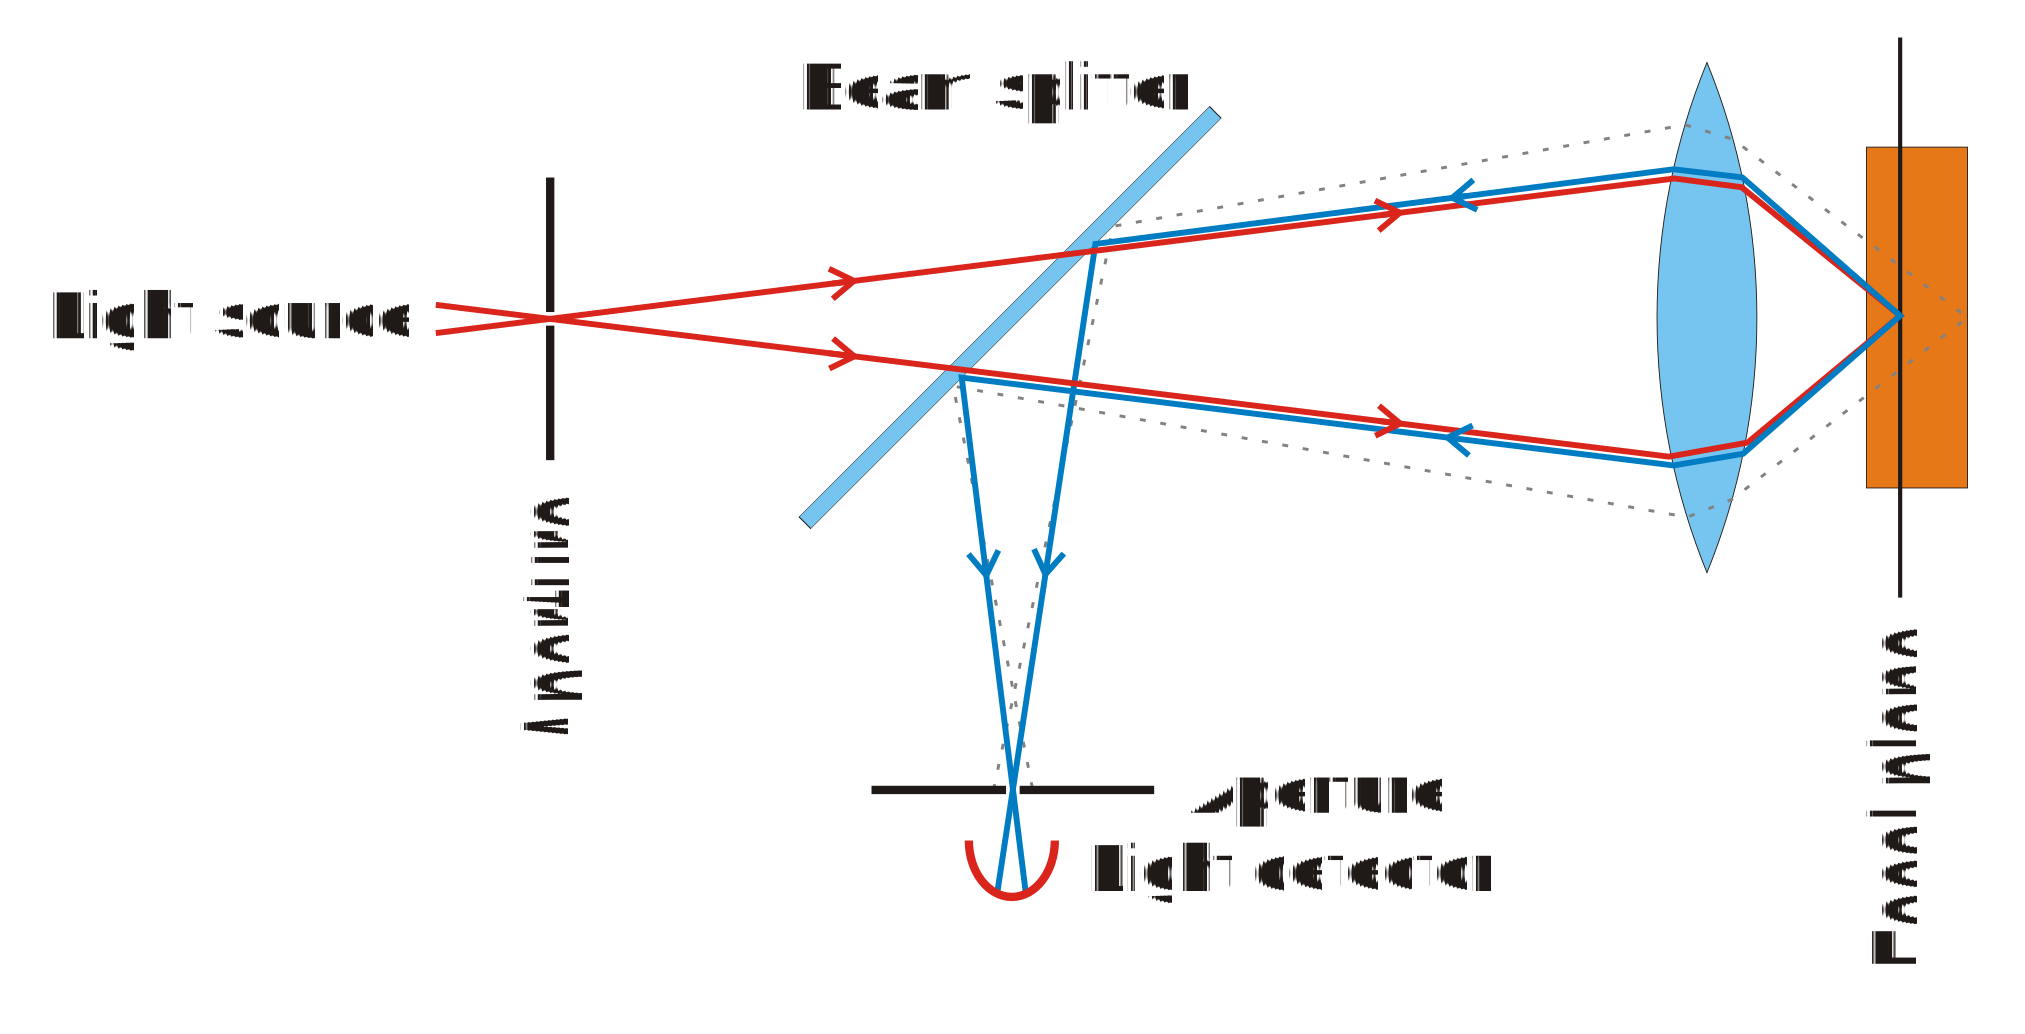
\includegraphics[width=0.95\textwidth]{pictures/ConfocalPrinciple}
\end{center}
\caption{Confocal microscope principle
(source:\href{http://en.wikipedia.org/wiki/File:Confocalprinciple.svg}{Wikipedia
})}
\label{fig:ConfocalPrinciple}
\end{figure}

\begin{figure}[htb]
\begin{center}
\leavevmode
 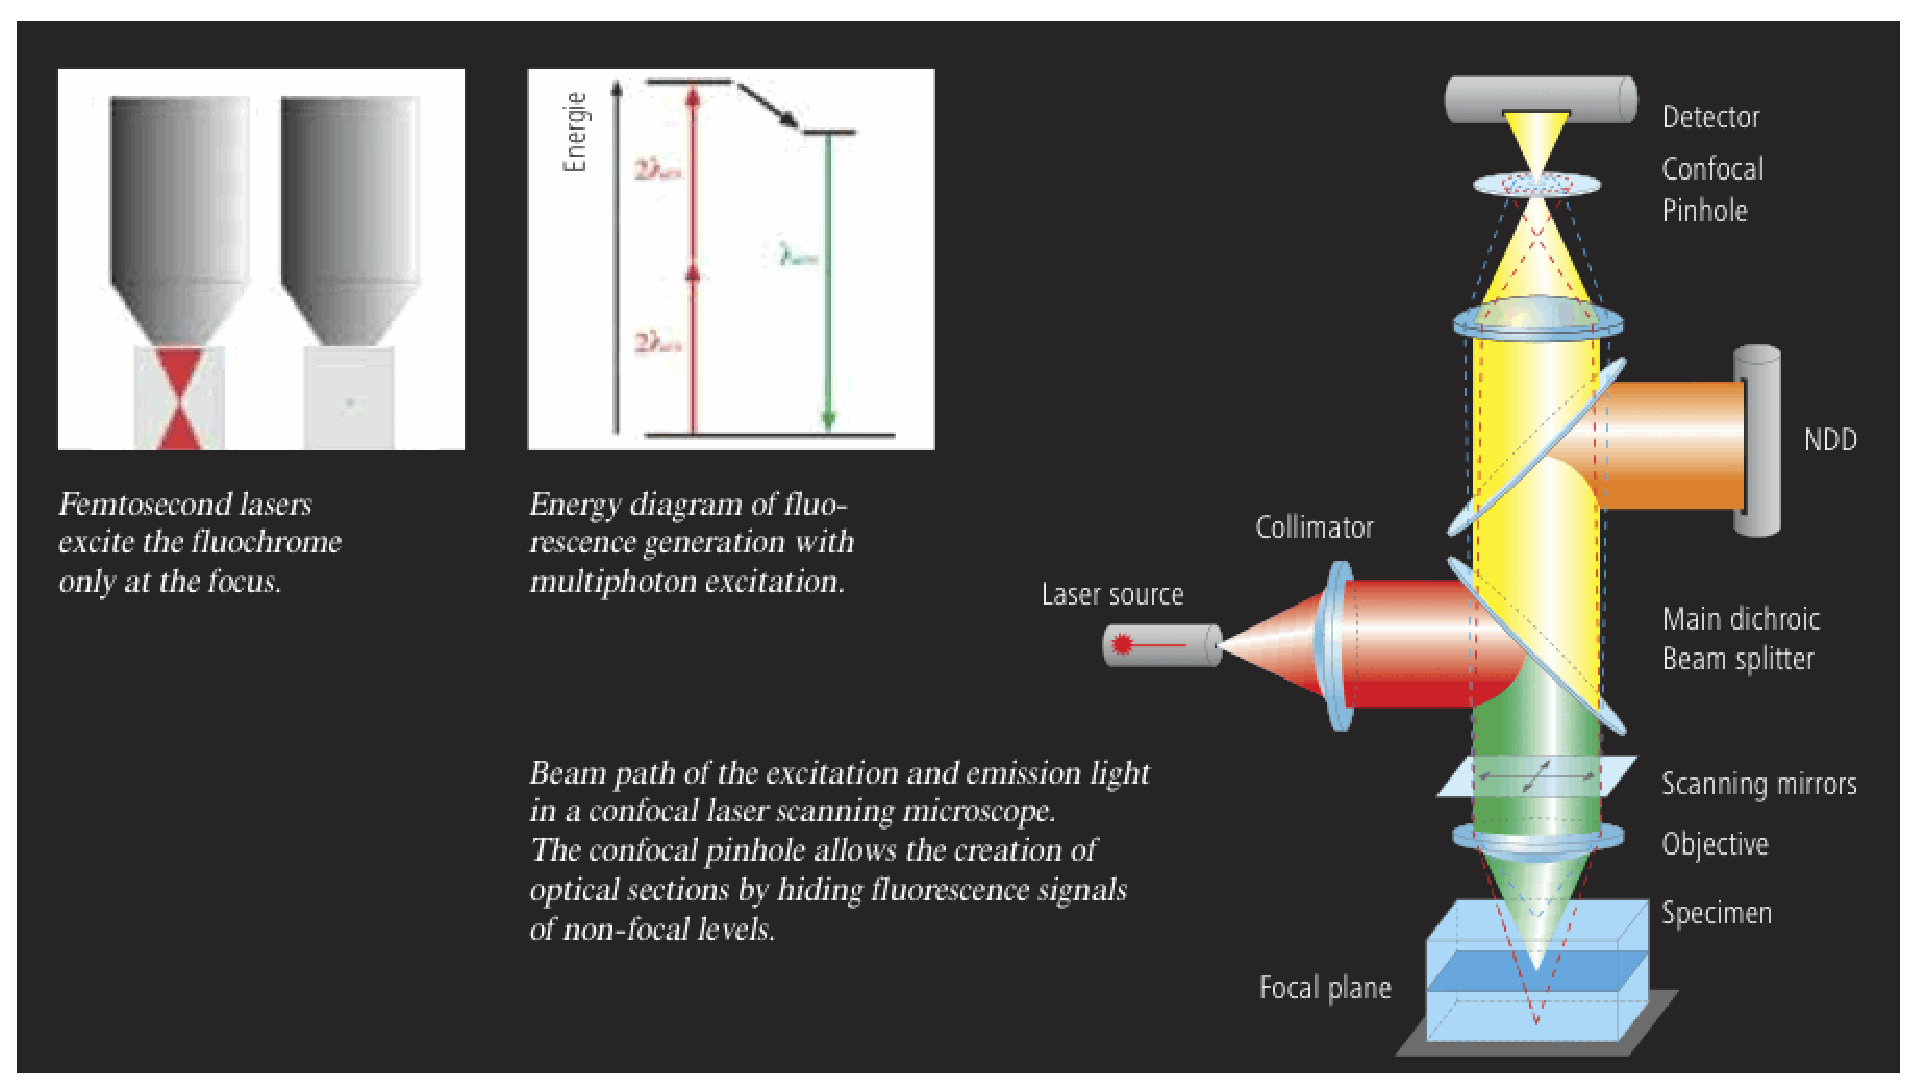
\includegraphics[width=0.95\textwidth]{pictures/ConfocalZeissPrinciple}
\end{center}
\caption{2-photon confocal microscope principle (Zeiss documentation)}
\label{fig:Confocal2photonsPrinciple}
\end{figure}

\begin{figure}[htb]
\begin{center}
\leavevmode
 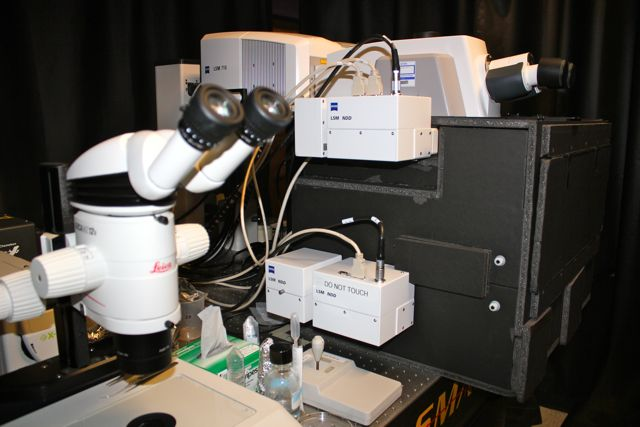
\includegraphics[width=0.95\textwidth]{pictures/PICmicroscope}
\end{center}
\caption{2-photon confocal microscope Zeiss 710 NLO in service in the Megason
Lab}
\label{fig:MicMegason}
\end{figure}

%%%%%%%%%%%%%%%%%%%%%%%%%%%%%%%%%%%%%%%%%%%%%%%%%%%%%%%%%%%%%%%%%%%%%%%%%%%%%%%
%%%%%%%%%%%%%%%%%%%%%%%%%%%%%%%%%%%%%%%%%%%%%%%%%%%%%%%%%%%%%%%%%%%%%%%%%%%%%%%
%%%%%%%%%%%%%%%%%%%%%%%%%%%%%%%%%%%%%%%%%%%%%%%%%%%%%%%%%%%%%%%%%%%%%%%%%%%%%%%

\subsection{Image Processing}

After the embryos have been labeled and imaged, the final challenge of in toto
imaging is image processing. The goal of image processing is to track all the
cell movements and divisions to generate cell lineage trees, to define the
boundaries of all cells and their compartments (nucleus, cytoplasm, membrane,
extracellular space), and to quantize the level of fluorescence within each
cell and subcellular compartment.\\

In order to process all the acquired data, an image processing team of
is working on the next platform of microscopy images analysis: {\gofigure}.
Their goal is to create a very accessible "cross-platform"\footnote{In
computing, cross-platform, or multi-platform, is
an attribute conferred to computer software or computing methods and concepts
that are implemented and inter-operate on multiple operating systems and
hardware.}, "open-source"\footnote{of or
relating to or being computer software for which
the source code is freely available, but which use may be restricted by a
license.}, freely distributed, application with a high quality code, for
biologists to process their data and for computer scientists and image
processing specialists the opportunity to promote their methods.

%%%%%%%%%%%%%%%%%%%%%%%%%%%%%%%%%%%%%%%%%%%%%%%%%%%%%%%%%%%%%%%%%%%%%%%%%%%%%%%
%%%%%%%%%%%%%%%%%%%%%%%%%%%%%%%%%%%%%%%%%%%%%%%%%%%%%%%%%%%%%%%%%%%%%%%%%%%%%%%
%%%%%%%%%%%%%%%%%%%%%%%%%%%%%%%%%%%%%%%%%%%%%%%%%%%%%%%%%%%%%%%%%%%%%%%%%%%%%%%


\subsection{Biological data analysis}

Biologists acquire tremendous amount of data (see table~\ref{tab:DataSizes})
corresponding in three dimensional videos of zebra fishes embryos
(see figure~\ref{fig:fig:embryoConfocalSlice}).

\begin{figure}[htb]
\begin{center}
\leavevmode
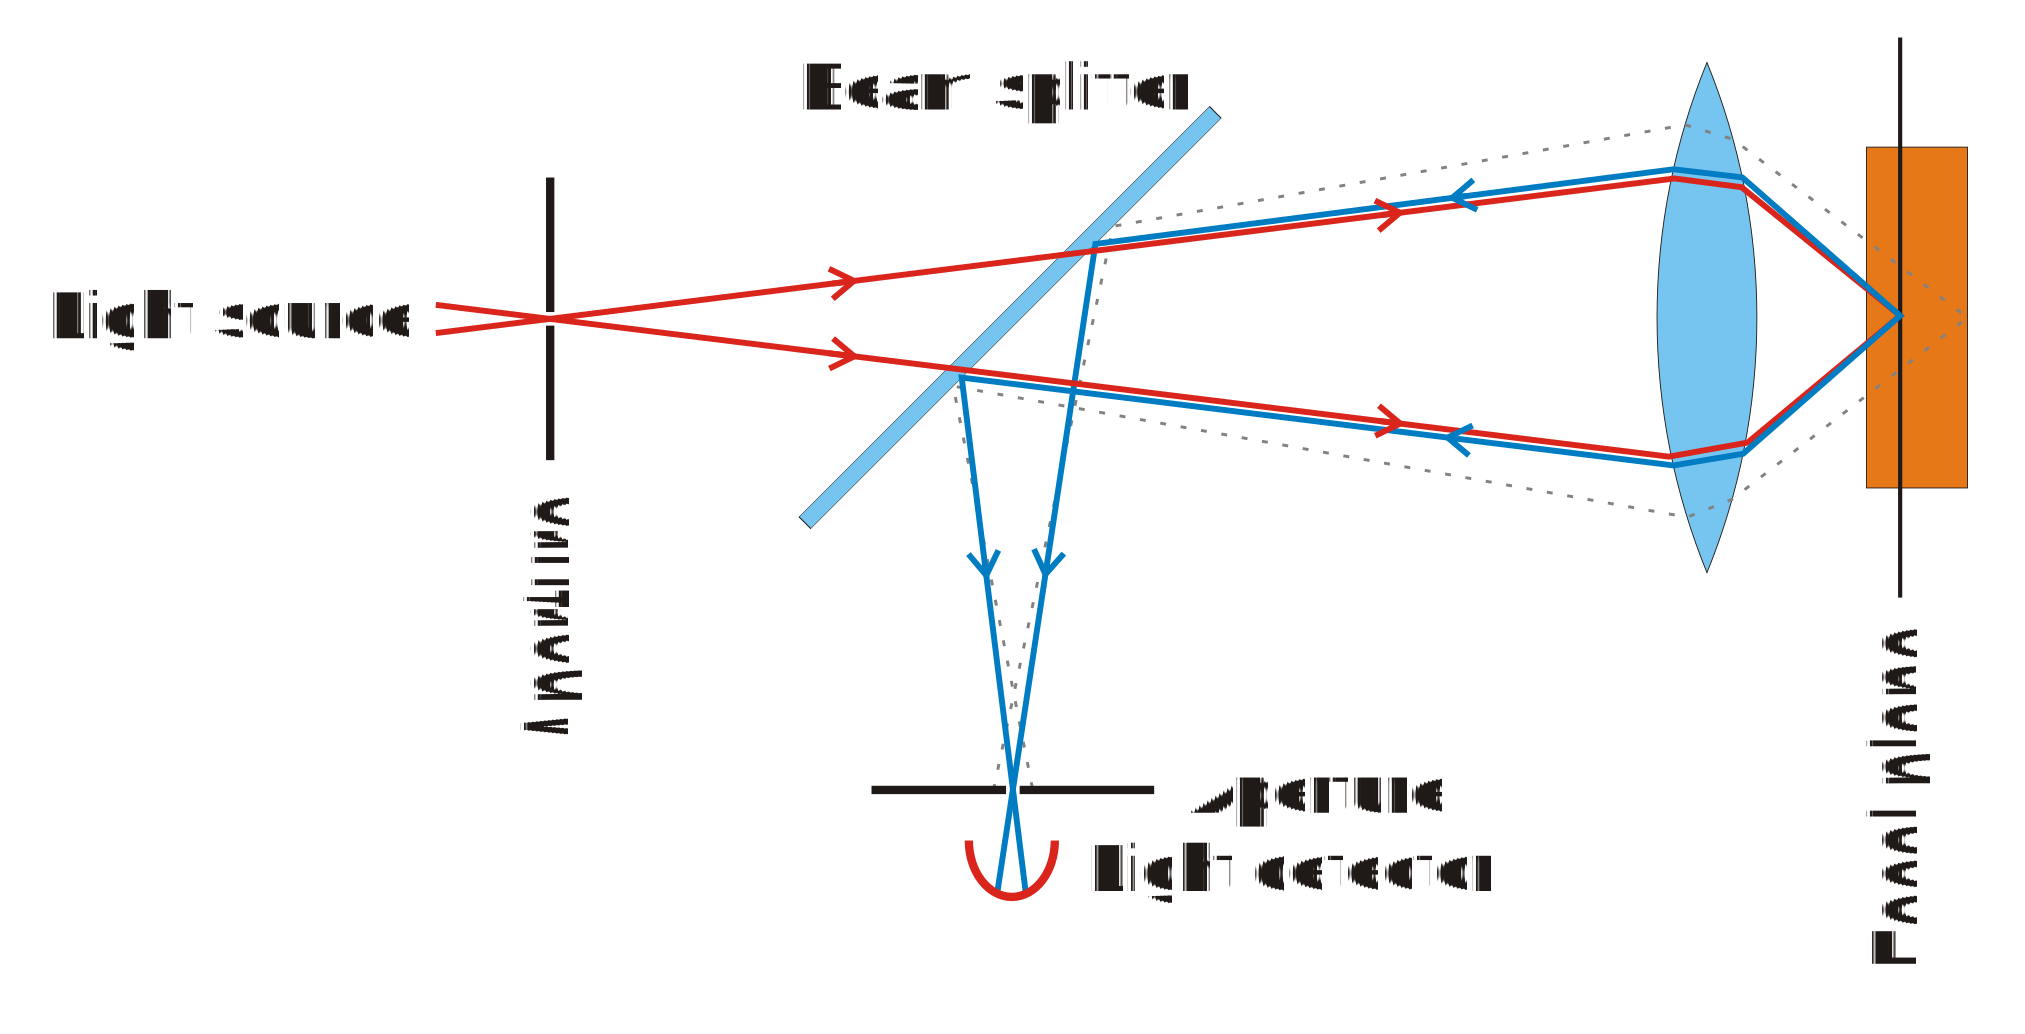
\includegraphics[width=0.95\textwidth]{pictures/ConfocalPrinciple}
\end{center}
\caption{Confocal microscope principle (source:\href{http://en.wikipedia.org/wiki/File:Confocalprinciple.svg}{Wikipedia})}
\label{fig:ConfocalPrinciple}
\end{figure}

\begin{figure}[htb]
\begin{center}
\leavevmode
 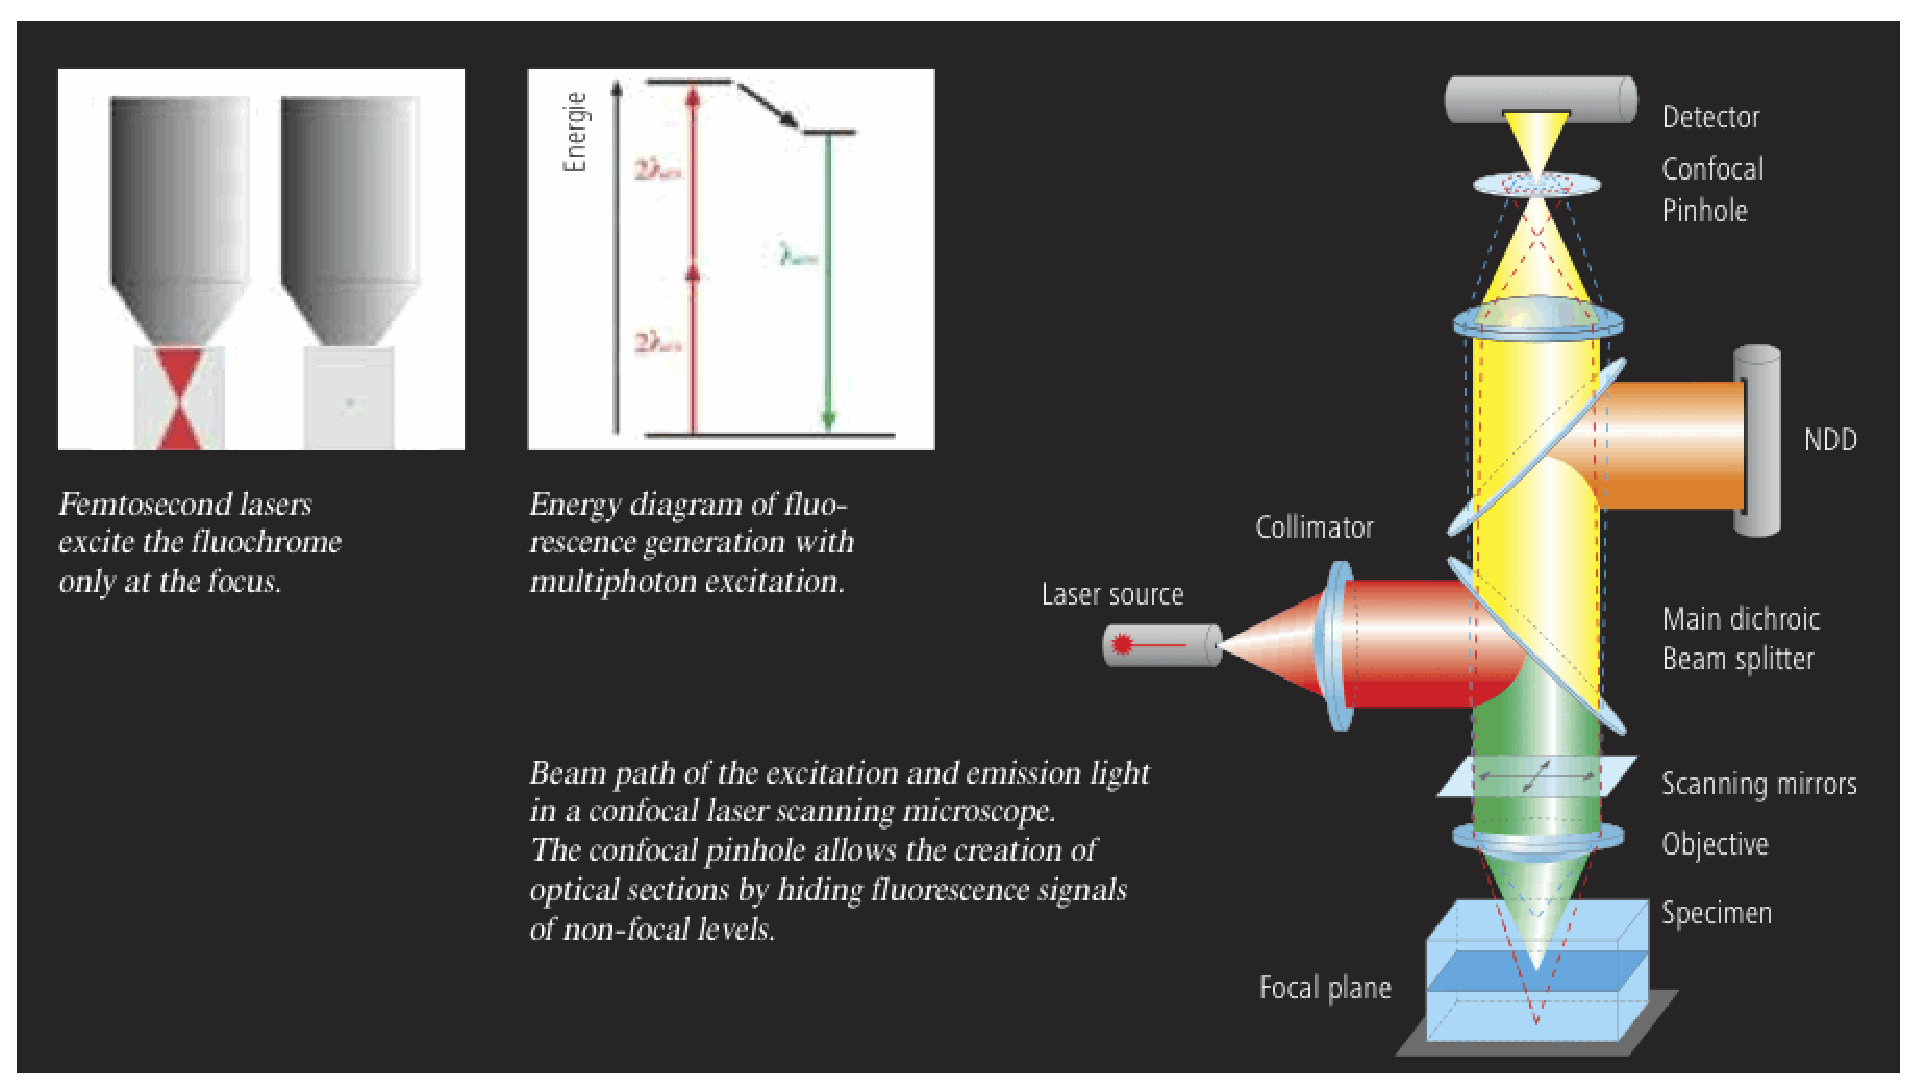
\includegraphics[width=0.95\textwidth]{pictures/ConfocalZeissPrinciple}
\end{center}
\caption{2-photon confocal microscope principle (Zeiss documentation)}
\label{fig:Confocal2photonsPrinciple}
\end{figure}

\begin{figure}[htb]
\begin{center}
\leavevmode
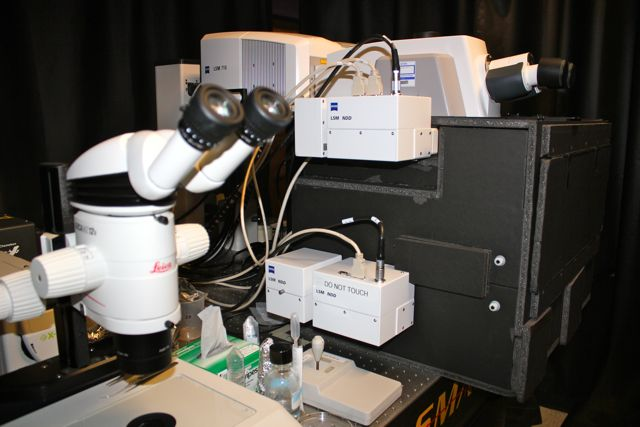
\includegraphics[width=0.95\textwidth]{pictures/PICmicroscope}
\end{center}
\caption{2-photon confocal microscope Zeiss 710 NLO in service in the Megason Lab}
\label{fig:MicMegason}
\end{figure}

\clearpage

\section{Challenges of data sets to be processed}

\subsection{Large amount of data}
\subsection{tout ce qui est complique}

\section{Problematic}

Here What's the problem you want to solve

% % Chapitre sur le rapport de recherche :


\chapter{Research report} 


\section{Problematic}


I mainly focused on membrane segmentation prior to arriving in the Megason lab. This is a challenging problem, as shown by the data analysis : the membrane data is incomplete, noisy, three dimensional and anisotropic.

Having no prior knowledge on Kishore's data denoising, I focused on level sets techniques to segment the membrane.
The level set theory provides a very flexible framework for segmentation problems. They are easily extensible to any dimension.
The drawbacks are that they are computationally intensive, and that the topology of the segmented region is by principle not controlled.

Similarly to region growing algorithms, level set algorithms can be initialized to provide prior information.
I focused on growing a levelset function from cells center. For that purpose, we need a good cell localization.
I have been studying levels sets in Creatis, for the purpose of cell segmentation and had some results in two dimensions.
I was then considering that nuclei were already correctly detected and segmented.
But when i arrived in the Megason Lab, I realized that before trying to segment the membrane using the techniques I studied in Creatis, I would need a correct cell nuclei detection.
We decided with Kishore that there was improvements to be brought to the cell nuclei detection algorithms.

That's why I started being interested in the problem of nuclei detection, in 3D confocal data.
After experiencing with Kishore's techniques, I implemented a recent algorithm for comparison, and proposed a new technique, with Dr Arnaud Gelas.


\chapter{My Proposals}
\chapter{Results}

%
%\section*{Introduction}
%
%\subsection*{}
%
%\TODO{elle pue cette intro}
%I am presenting in this chapter, the research project I have been working on during the PFE. I have first undergone a bibliographic step, to acquire knowledge about the matter. Thanks to this research, I could determine which problems are still to be solved. Then I tried to find appropriate solutions to the problems encountered.
%
%The main difficulty in research, is that very often, there is no solution yet to the problem, in the domain. Therefore, I have had to do a bibliography, in order to determine the state of the art, and eventually learn some new theories.
%
%The image processing domain is particular: many algorithms are invented and published, but very few are available nor applicable to diverse images.
%Thus, there is a re-programming and evaluation step, prior to any innovation.

\subsection*{}

While in the Megason Lab, I have been working on segmenting fluorescent microscopy images.
Datas are four-dimensional (space and time), and represent regions (ear, brain...) of a developing zebrafish.
It is possible to visualy distinc nuclei and membranes of cells. Those elements constitute the basis of the model that we try to create.
Therefore, we have to be able to detect and track every cell across time. The model will also have to integrate morphological informations of each cell.

The creation of this model is a thesis subject : cells lineage registration in microscopy, during which I would like to extend my work.

Prior to arriving in the laboratory, I have been working on cell membrane. I have then concentrated my researches on cell nuclei detection and localization.




%
%  STATE OF THE ART
%

\section{State of the art in the megason lab}

\subsection{The Megason lab imaging pipeline}

Dr Kishore Mosaliganti has been working for two years in the Megason lab, in order to develop new segmentation methods for fluorescent images.
He has been working on experiencing and developing diverse algorithms for nuclei and membrane detection and segmentation.
As presented is the previous section, the datasets in the Megason Lab are extremely challenging:
they are huge and present important drawbacks (resolution, noise) as they are provided for visual processing and not computer assisted processing.

As these datasets are very big, and four dimensional, it is not possible to use Matlab for easy prototyping and experiencing : 
most of the time, the very low resolution third dimension will considerably modify the results.
There is also a time issue : the datasets must be treated in an acceptable amount of time,
and that prevents us from using Matlab language that does not provide every optimized function that we need for 3D images visualization and processing.
This forces us to program and prototype in {\C++}. The standard library used for image processing in the Megason Lab is ITK. Kishore's algorithm are all coded with this library.
The data processing in ITK is represented by pipelines : a series of connected filters that perform image processing tasks.
The Megason lab aslo develops a visualization program for microscopy data: {\gofigure}. This program uses ITK and VTK for processing and visualization of data. The long term goal being to include the algorithms to {\gofigure}, we also have to use those libraries.

Kishore studied several pipelines for nuclei and membrane segmentation.
For nuclei segmentation, an approach based on detection of nuclei, and region growing with the level set theory was used last year.
This year, a new approach based on nuclei detection and watershed algorithms is being used.
The algorithm used are standard and contour based for the detection of nuclei.
This leads to many errors in detection, due to the poor image quality. Right now, these errors are compensated after the segmentation step.

For membrane segmentation, Kishore is proposing a very good denoising technique based on anisotropic diffusion and tensor voting.
The reconstruction of the membrane structure is effective, even in low quality images. A segmentation step has to be implemented on top of it.


%
%  SEEDING
%


\section{Cell nuclei detection}

Cell nuclei shapes varies from spherical to curved ellipsoidal. As introduced above, the microscopy images are challenging, they are very noisy and anisotropic.
The main encountered difficulty is clustered nuclei that result from the point spread function of the microscope and the low resolution in the third dimension.

The algorithms used in the Megason lab for nuclei and membrane segmentation are based on an initialisation inside the nuclei.
Right now, a composite algorithm is used for detecting these nuclei based on a combination of contour based algorithms (see~\ref{sect:megasonExisting}).
This method gives good enough results for starting a watershed algorithm. Segmented regions that obviously don't correspond to a cell nucleus are eliminated. The final result of the segmentation process is evaluated.
\TODO{cite Kishore papers}


This is clear that  the nuclei detection has to be improved.
I started by carying a bibliographic research, to determine the state of the art in the nuclei segmentation/detection domain.
Then, I implemented a new algorithm based on the Laplacian of Gaussian method.
After that, I created an evaluation framework, to compare the results given by this new algorithm, and Kishore's.
We finally proposed a new method taking advantage of the cell membrane information.



\subsection{Existing methods}

There are several papers dealing with cell nuclei or cell detection 
\cite{loukas2003image,umesh2001efficient,al2009improved},
but only one is based on 3D confocal images~\cite{li20073}, similar to the ones acquired in the Megason lab.

\subsubsection*{Confocal nuclei detection}
G. Li {\etal}~\cite{li20073}, describe a segmentation method for nuclei in 3D confocal datasets. The method they use is based on gradient vector flow tracking.
The image processing pipeline is presented figure~\ref{fig:gradientflowFlowchart}.
\begin{description}
  \item[Data] are 3D confocal datasets from zebrafish embryos. They are fluorescent nuclei.
  \item[Method] is described figure~\ref{fig:gradientflowFlowchart}. 
  A re-sampling and spline based interpolation is performed on the original data to get isotropic datasets.
  The gradient vector diffusion field (see figure~\ref{fig:gradientflowFlowfield}) is then computed on a Gaussian blurred version of the isotropic data.
  Following \cite{bajcsy1989multiresolution}, an elastic constraint is added to the diffusion equation to get a smooth vector field.
  The tracking consists in selecting some points and moving them according to the vector field. The resulting trajectories end in "sinks" that correspond to center of nuclei.
  A refinement step groups the close "sinks".
  The segmentation is the done by cropping the image around each nuclei and applying a local adaptive threshold to find one nuclei per subregion.
  A final step consists in eliminating the false positives (nuclei which are too small).
  \item[Evaluation] is performed on 10 confocal datasets. The mean amount of nuclei in the datasets is 310. The number of over segmented and under segmented nuclei is presented. The automatic segmentation result is compared with the segmentation of two experts.
  \item[Results] the algorithm provides good results in the paper: 
  4.93\% of over-segmented nuclei,
  and 5.03\% of under-segmented nuclei.
  \item[Comments]:
  The article misses the part describing the region cropping for getting the regions where the adaptive
   threshold should be computed.
   Looking at the illustration, it seems like these regions are either determined
   according to attraction basins of each sink, or with a constrained Voronoi diagram.
\end{description}
\begin{figure}[h]
\begin{center}
\leavevmode
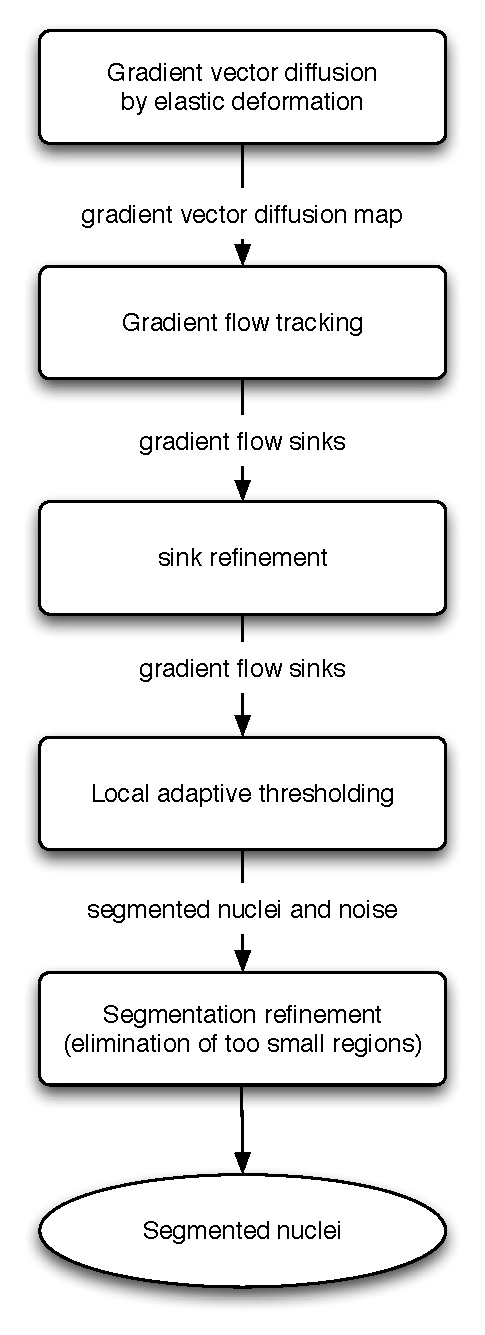
\includegraphics[height=0.75\textheight]{pictures/gradientflowFlowchart}
\end{center}
\caption{Flowchart of the algorithm proposed in~\cite{li20073}}
\label{fig:gradientflowFlowchart}
\end{figure}

\begin{figure}[h]
  \centering
  \captionsetup[subfloat]{labelformat=empty}
  \subfloat[][]{{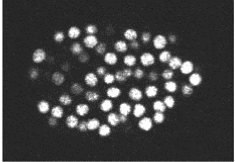
\includegraphics[width=0.33\textwidth]{pictures/gradientflowSegmenta}\label{fig:gradientflowSegmenta}}}
  \subfloat[][]{{
\includegraphics[width=0.33\textwidth]{pictures/gradientflowSegmentb}\label{fig:gradientflowSegmentb}}}\\
  \subfloat[][]{{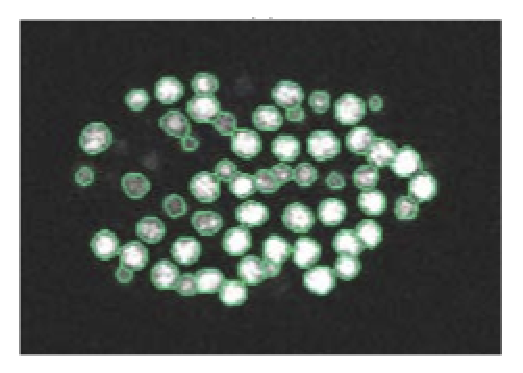
\includegraphics[width=0.33\textwidth]{pictures/gradientflowSegmentc}\label{fig:gradientflowSegmentc}}}
  \subfloat[][]{{
\includegraphics[width=0.33\textwidth]{pictures/gradientflowSegmentd}\label{fig:gradientflowSegmentd}}}
\caption{%
Illustration of 3D cell nuclei segmentation on a 2D slice, from~\cite{li20073}.
\subref{fig:gradientflowSegmenta}: A slice from 3D cell nuclei image;
\subref{fig:gradientflowSegmentb}: Boundaries of small regions overlaid on the slice;
\subref{fig:gradientflowSegmentc}: Edges of cell nuclei overlaid on the slice after the step of adaptive thresholding;
\subref{fig:gradientflowSegmentd}: Randomly color-coded extracted cells.}
\end{figure}

\begin{figure}[h]
  \centering
  \captionsetup[subfloat]{labelformat=empty}
  \subfloat[][]{{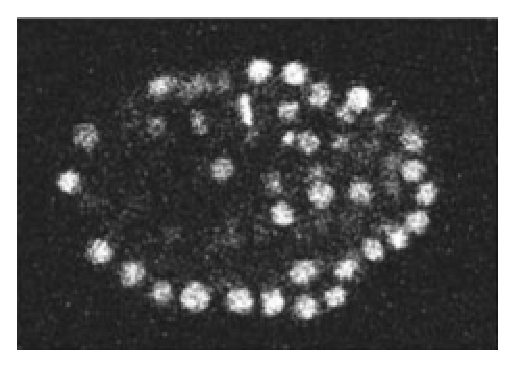
\includegraphics[width=0.5\textwidth]{pictures/gradientflowFlowfielda}\label{fig:gradientflowFlowfielda}}}\\
  \subfloat[][]{{
\includegraphics[width=0.33\textwidth]{pictures/gradientflowFlowfieldb}\label{fig:gradientflowFlowfieldb}}}
  \subfloat[][]{{
\includegraphics[width=0.33\textwidth]{pictures/gradientflowFlowfieldc}\label{fig:gradientflowFlowfieldc}}}\\
  \subfloat[][]{{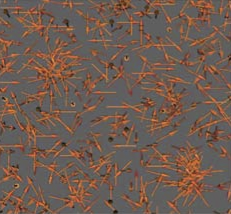
\includegraphics[width=0.33\textwidth]{pictures/gradientflowFlowfieldd}\label{fig:gradientflowFlowfieldd}}}
  \subfloat[][]{{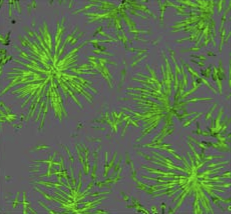
\includegraphics[width=0.33\textwidth]{pictures/gradientflowFlowfielde}\label{fig:gradientflowFlowfielde}}}
\caption{%
The 3D view of gradient vector field and diffused gradient vector field with elastic deformation transformation of a slice cropped from a 3D cell nuclei image, from~\cite{li20073}.
\subref{fig:gradientflowFlowfielda}: A slice of the 3D image;
\subref{fig:gradientflowFlowfieldb}: The original gradient vector field;
\subref{fig:gradientflowFlowfieldc}: The diffused gradient flow field with elastic deformation transformation;
\subref{fig:gradientflowFlowfieldd}: Zoomed view of \subref{fig:gradientflowFlowfieldb};
\subref{fig:gradientflowFlowfielde}: Zoomed view of \subref{fig:gradientflowFlowfieldc}.}
\end{figure}
\clearpage

\subsubsection*{3D histological pathological cell detection}
 P.S. Umesh Adiga {\etal}~\cite{umesh2001efficient}, present a method for segmenting cells in histological images 
  (which are somehow close to nuclei in fluorescent images).
  \begin{description}
  \item[Data] are 3D confocal histo-pathological images of cells in thick tissues.
  \item[Method] is described figure~\ref{fig:watershedFlowchart}.
  A first step consists in thresholding the image to keep only the nuclei. The threshold level is given by an empirical law based on the histogram of the images.
  Then, a succession of mathematical morphology operations consisting in opening and closing with a structuring element of same size, are used to improve the data. 
  This filters the texture of the cells, and removes holes.
  An intensity correction is then applied along the z axis. The figure~\ref{fig:watershedPrefilt} illustrates the results of this pre-processing.
  After a binarization of the preprocessed image, a distance map is computed and thresholded to find the cell markers, to initiate the watershed algorithm.
  Once the watershed algorithm has converged, a region merging process groups over-segmented cells. The region merge used in this paper is described by figure~\ref{watershedMerge}.
  \item[Evaluation] is performed on 15 3D datasets. The mean amount of nuclei in the datasets is 22. The information provided by the evaluation is the number of detected cells compared to the number of real cells present. No information is given on the type of error. The algorithm is compared to \cite{malpica1997applying}, and shows better performance according to the evaluation criterion.
  \item[Results] the algorithm provides very good results in the paper with 2\% of error instead of 9\% for \cite{malpica1997applying}.
  \item[Comments]: this article is well presented with a description of all the steps of the processing pipeline.
  The evaluation is done on small datasets (256*256*24) with few cells. A good information would have been amount of under segmented cells. 
\end{description}
\begin{figure}[h]
\begin{center}
\leavevmode
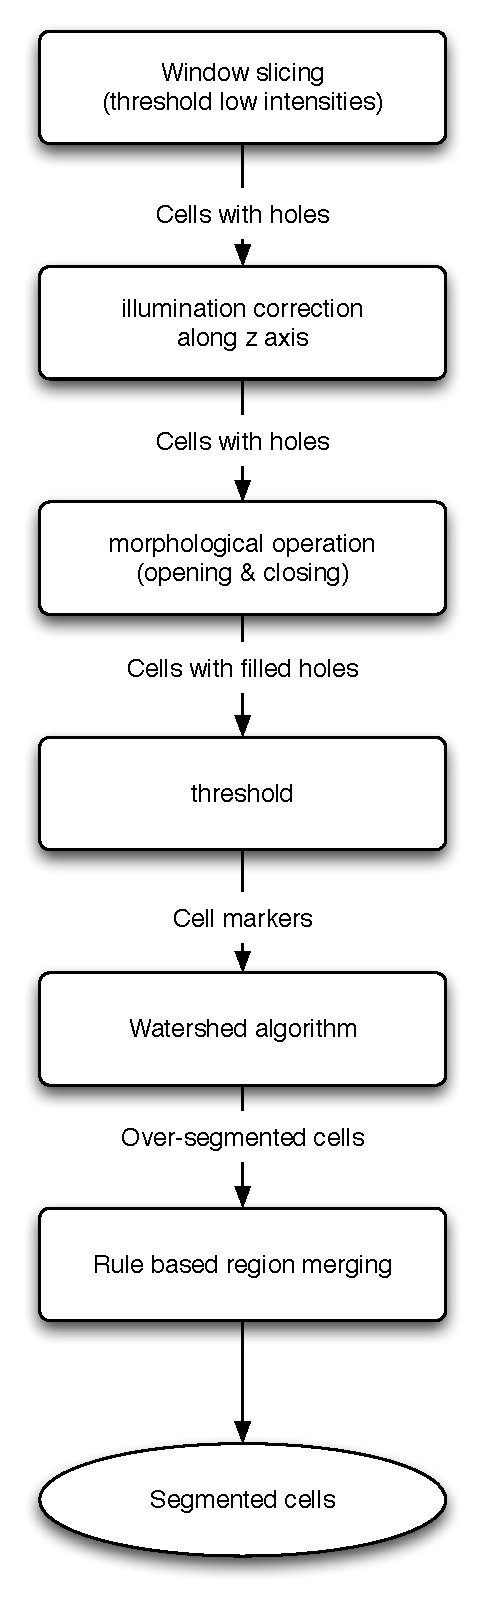
\includegraphics[height=0.75\textheight]{pictures/watershedFlowchart}
\end{center}
\caption{Flowchart of the algorithm proposed in~\cite{umesh2001efficient}}
\label{fig:watershedFlowchart}
\end{figure}
\begin{figure}[h]
  \centering
  \captionsetup[subfloat]{labelformat=empty}
  \subfloat[Diagrammatic representation of detecting the small fragments of the object and finding its parent.]{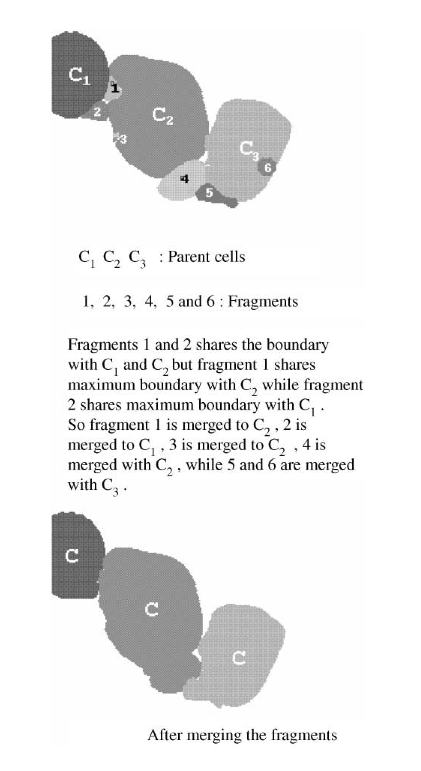
\includegraphics[width=0.49\textwidth]{pictures/watershedMerge}\label{fig:watershedMerge}}
\subfloat[Result of image enhancement steps shown over a single image slice: (a) original image slice, (b) result of window slicing, (c) result of size-filtering, (d) result of morphological opening and closing of a 3D image.]{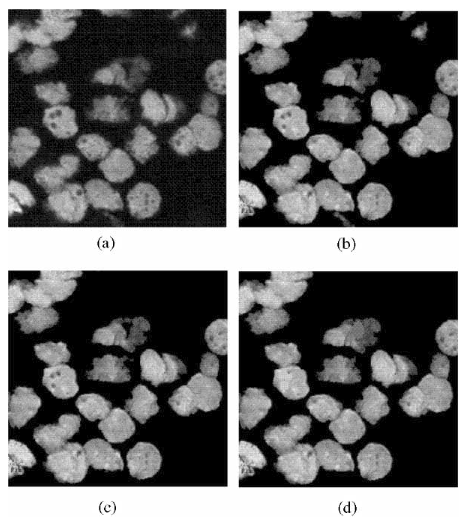
\includegraphics[width=0.49\textwidth]{pictures/watershedPrefilt}\label{fig:watershedPrefilt}}
\caption{illustrations from \cite{umesh2001efficient}}
  \label{fig:watershedIllustration}
\end{figure}
\clearpage


\subsubsection*{Histological cell nuclei detection}
\label{sect:farsight}
Yousef Al-Kofahi {\etal}~\cite{al2009improved}, presents a new method for nuclei detection.
  \begin{description}
  \item[Data] are 2D histological images (see figure~\ref{fig:farsightInitial}).
  \item[Method] is described figure~\ref{fig:farsightFlowchart}.
  A first step consists in finding the foreground of the image with a graph cut based binarization (illustrated figure~\ref{farsightBinary}).
  A distance map is then computed on this binary image, and is used to constrain the scales of a multiscale Laplacian of Gaussian (see~\ref{sect:MLOG}).
  The original image is processed by the scale-constrained multi-scale Laplacien of Gaussian.
  A local maxima detection is performed on the resulting scalar field (as shown figure~\ref{fig:farsightMLOG}).
  Those local maximas correspond to the position of the cell.
  A watershed algorithm is then initiated from these points, and finally refined by manual editing and "alpha-refinement".
  \item[Evaluation] is done on 25 images containing an average of 298 cells per image. The results present the number of over and under segmented cell nuclei and separates encroachment errors.
  \item[Results] the algorithm provides acceptable results : 13.7\% of error.
  \item[Comments]: this article is well presented with a description of all the steps of the processing pipeline.
  The evaluation is done on enough images, and the results are detailed.
  The algorithm was implemented in the Farsight toolkit (FTK, \url{http://www.farsight-toolkit.org/}), but we were unable to make it run on 3D data.
\end{description}
\begin{figure}[h]
\begin{center}
\leavevmode
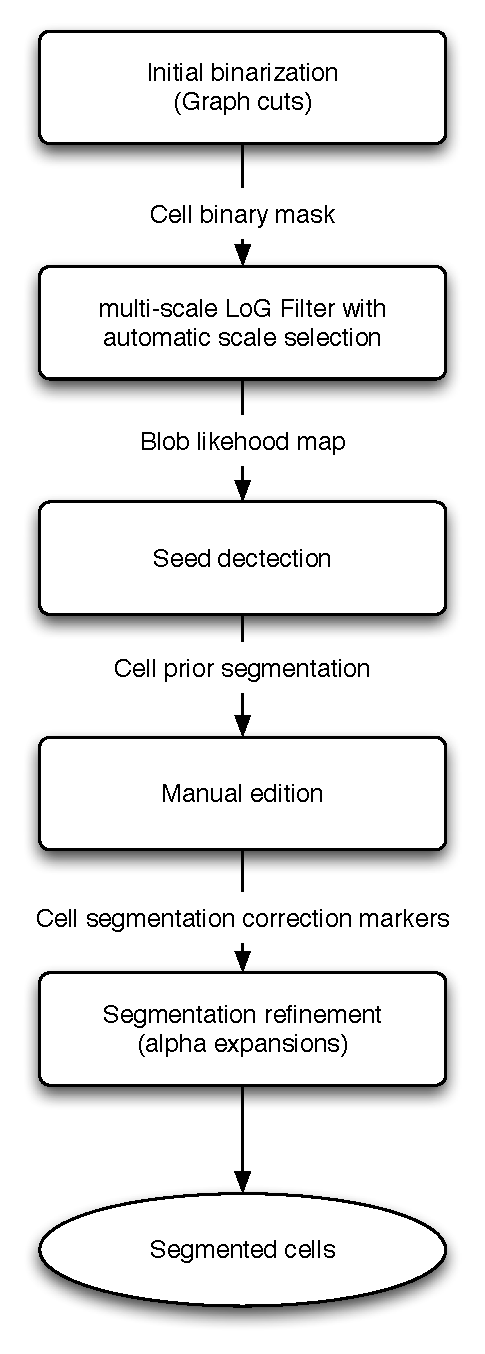
\includegraphics[height=0.75\textheight]{pictures/farsightFlowchart}
\end{center}
\caption{Flowchart of the algorithm proposed in~\cite{al2009improved}}
\label{fig:farsightFlowchart}
\end{figure}
\begin{figure}[h]
  \centering
  \captionsetup[subfloat]{labelformat=empty}
\subfloat[(A) Nuclear channel from spectral unmixing.]{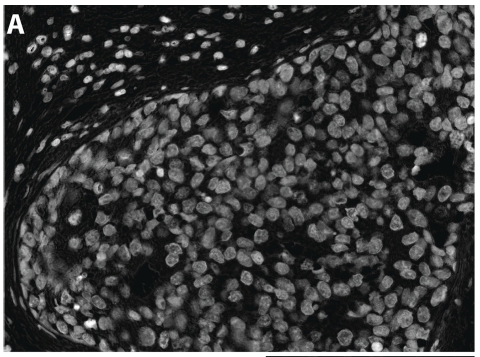
\includegraphics[width=0.49\textwidth]{pictures/farsightInitial}\label{fig:farsightInitial}}
\subfloat[(B) Foreground extraction results. Pixels marked yellow represent a large connected component.]{
\includegraphics[width=0.49\textwidth]{pictures/farsightBinary}\label{farsightBinary}} \\
\subfloat[(C) Surface plot of the multiscale LoG filtering results for a small region. (D) Initial segmentation based on the LoG. (E) Surface plot of the distance-map-constrained multiscale LoG. (F) Improved initial segmentation resulting from the distance-constrained LoG.]{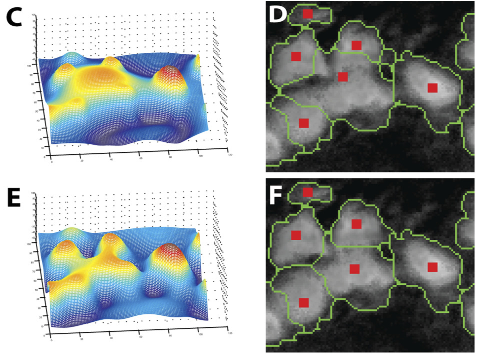
\includegraphics[width=0.75\textwidth]{pictures/farsightMLOG}\label{fig:farsightMLOG}}
\caption{illustrations from \cite{al2009improved}}
  \label{fig:farsightIllustration}
\end{figure}
\clearpage


%
%%\subsubsection*{Loukas two observers}
%%
%% C.G. Loukas {\etal}~\cite{loukas2003image}, published an article about automatic counting of cancer cell nuclei in tissue sections.
%%As their data is very different from ours, the main interest of this article is the evaluation method based on based on two observers.
%%  They count the number of cells in ten images and the average number of cell counting error of the algorithm in percent the average number of cell present in the images is given (150). No information is provided on evaluating the cell nuclei position, or on the type of error : over detection or under detection ? The data are histological sections (2D).
%
%\begin{description}
%  \item[Data] are histological sections from cell cancers.
%  \item[Method] is based on a modified Laplacian of Gaussian filtering with maxima detector. The data being extremely different from ours, the method is not further described in this report.
%
%  \item[Evaluation] is performed on 10 confocal datasets. The mean amount of nuclei in the datasets is 310. The number of over segmented and under segmented nuclei is presented. The automatic segmentation result is compared with the segmentation of two experts.
%  \item[Results] the algorithm provides good results in the paper: 
%  4.93\% of over-segmented nuclei,
%  and 5.03\% of under-segmented nuclei.
%  \item[Comments]: this article is well presented and evaluated,
%  equations and references are given for algorithm reproduction.
%  A windows executable of the algorithm is also provided. The code source is not released though. 
%  The article misses the part desrcibing the region cropping for getting the regions where the adaptive
%   threshold should be computed. 
%   Looking at the illustration, it seems like these regions are either determined 
%   according to attraction basins of each sink, or with a constrained Voronoi diagram.
%\end{description}
%
%
%

\subsubsection{Existing method in the Megason Lab}
\label{sect:megasonExisting}
The existing method in the Megason Lab, for nuclei detection and segmentation, is also based on a detection of nuclei, and then, a segmentation, using watershed.
  \begin{description}
  \item[Data] are the challenging 3D confocal/2-photons images presented in the Data analysis part. 
  \item[Method] is described figure~\ref{fig:kishoreFlowchart},
  A pre processing stage consists in denoising the raw image, with an anisotropic diffusion filter.
  Then, the algorithm consists in a combination of methods : 
  hough transform, image masking and distance map, and the redial voting technique described in \cite{chang2007segmentation}, applied to the denoised image.
  Once the three filters processed the nuclei image, their output scalar fields are summed.
  A local maxima extraction is performed on this resulting field.
  This extraction filters the close local maximas, to reduce the noise impact, by selecting the highest local maxima, and ignoring the other local maximas in a certain radius.
  those maximas are then used for initializing a watershed algorithm.
  \item[Evaluation] has been visually carried out by Kishore, for the initialization points of the watershed.
  For the result of the watershed, the evaluation was performed on an expert-segmented dataset of 180 cell nuclei.
  \item[Results] are still to be evaluated.
  \item[Comments]: there is an existing method in the Megason lab, but it has not yet been evaluated nor published. Improving this method consists in, first going through the algorithms' code, then create a visualization and evaluation framework, and finally compare it with other methods.
\end{description}
\begin{figure}[h]
\begin{center}
\leavevmode
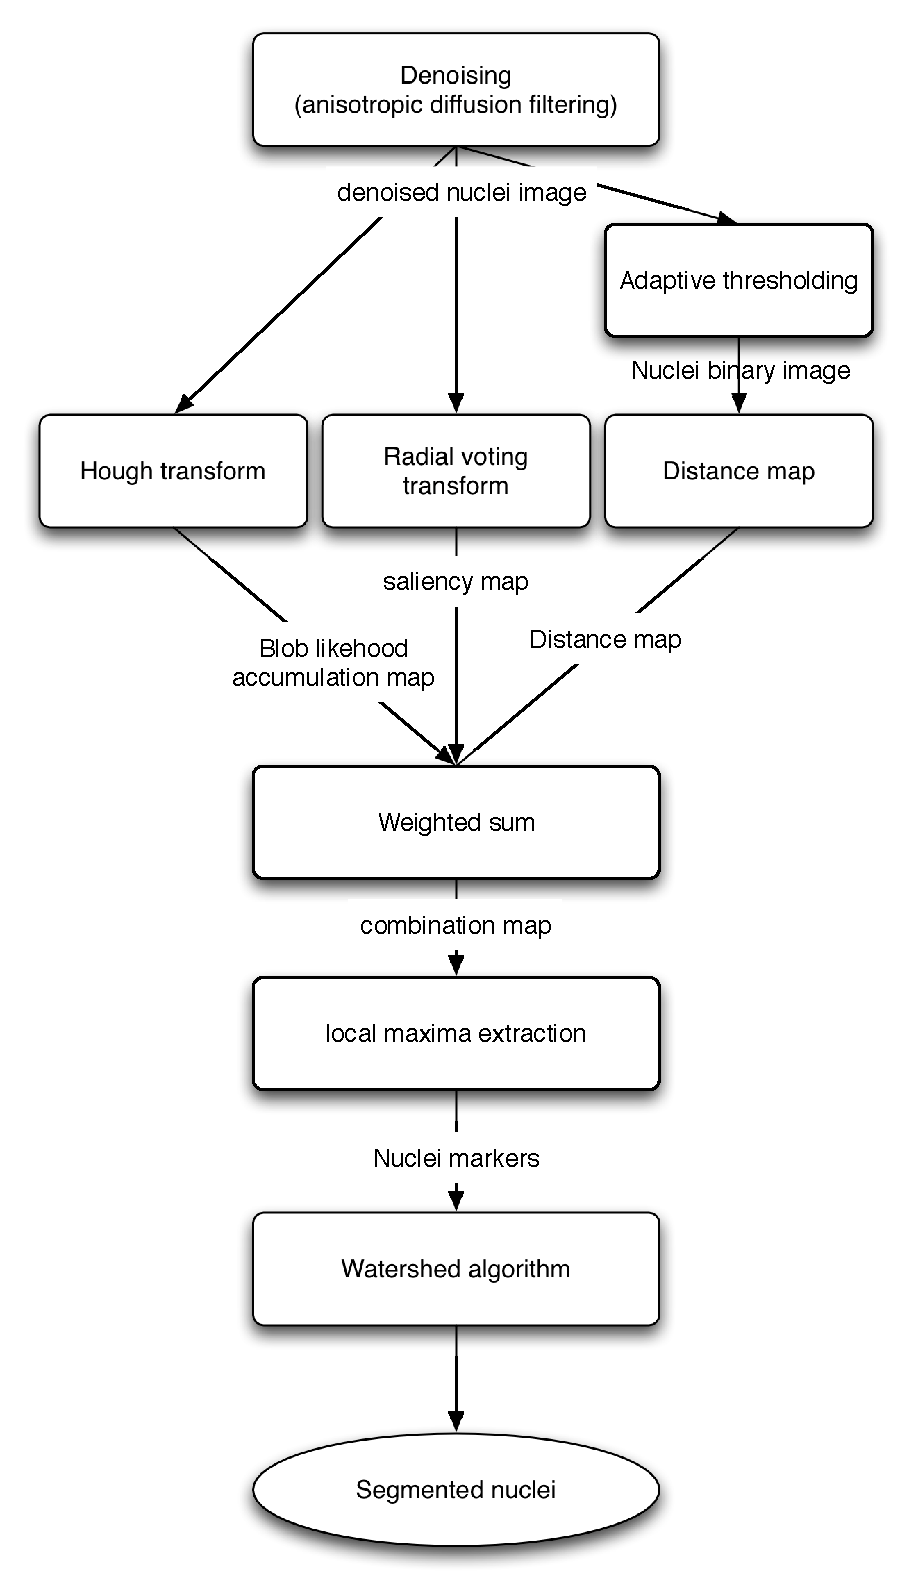
\includegraphics[height=0.75\textheight]{pictures/kishoreFlowchart}
\end{center}
\caption{Flowchart of the algorithm used in the Megason Lab}
\label{fig:kishoreFlowchart}
\end{figure}
\clearpage


\subsubsection*{Conclusion}

We can conclude that there are some existing algorithms for detecting and segmenting cell nuclei,
but very few were designed for 3D confocal data.
Most of the time, they perform well on 2D datasets, but are tricked by the low resolution of the third dimension.
The evaluation is most of times based on the final segmentation, and interesting informations are number of over/under-segmented cell nuclei.


\subsection{Proposal}
\label{sect:proposal}
There is still a lot of work to be done in order to improve the quality of nuclei detection. We propose here a new method based on the cell membrane information. We will first discuss the principle of this method, and then evaluate it on synthetic and real data.

\subsubsection{Principle}

\paragraph{preliminaries}

A Voronoi diagram is defined as such :
The Voronoi Cell of the site \( p \in P \) is given as follows


\TODO{complete voronoi equation if necessary}

All the papers we have been reading take advantage of the nuclei channel information, but none of them takes advantage of the membrane channel.
This channel provides capital information, especially in the case of stuck nuclei, where most common detection method fail.
Indeed, the membrane can separate the different nuclei.

\paragraph*{}

\begin{figure}[h]
\begin{center}
\leavevmode
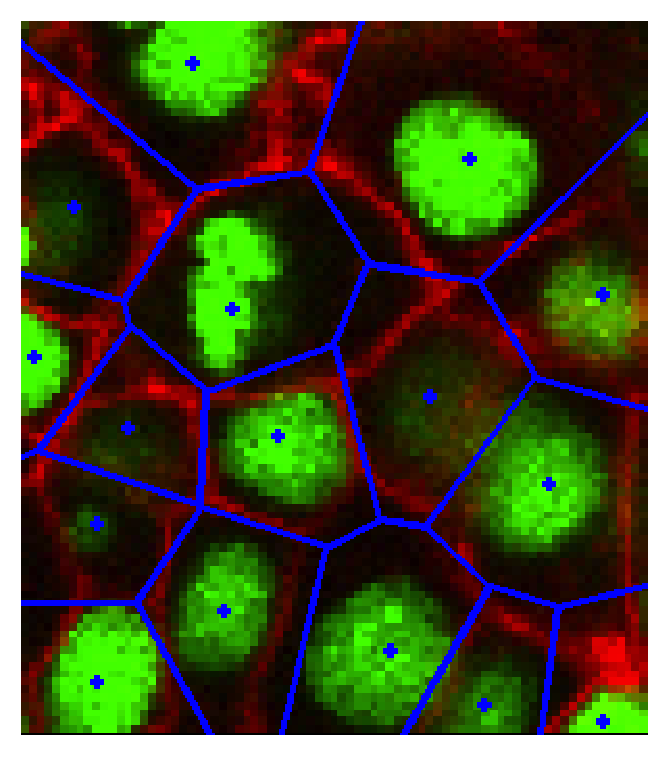
\includegraphics[width=0.5\textwidth]{pictures/voronoiExample2D}
\end{center}
\caption{Voronoi diagram (blue) centred in each cell nuclei (green), with the membrane (red)}
\label{fig:voronoiExample2D}
\end{figure}
Several article make use of Voronoi diagrams to delimiter the zone where one nuclei is present.
But the membrane is also around each nuclei. So the membrane channel provides us with information about nuclei positions.
We can see figure~\ref{fig:voronoiExample2D}, that the membrane can be approximated by a Voronoi diagram centred in each nucleus.
From this, we can use the membrane channel and consider it as a Voronoi tessellation, and from this, find the Delauney triangulation.
The triangulation's intersections would be the centres of the cells. And nuclei are most of times located next to the center of the cell.

\paragraph*{}



The Voronoi cells are constituted by all the points closer to the center of the cell than any other center. Thus, if we draw a distance map from the Voronoi cells, the local maximas of this distance map are the centres.
We want to take advantage of this principle by drawing a distance map on the membrane channel. For the localizing the local maximas, there is no need for a complete membrane information, as illustrated figure~\ref{fig:incompleteMembraneSynthetic}.
\begin{figure}[h]
  \centering
\subfloat[Synthetic Voronoi cell]{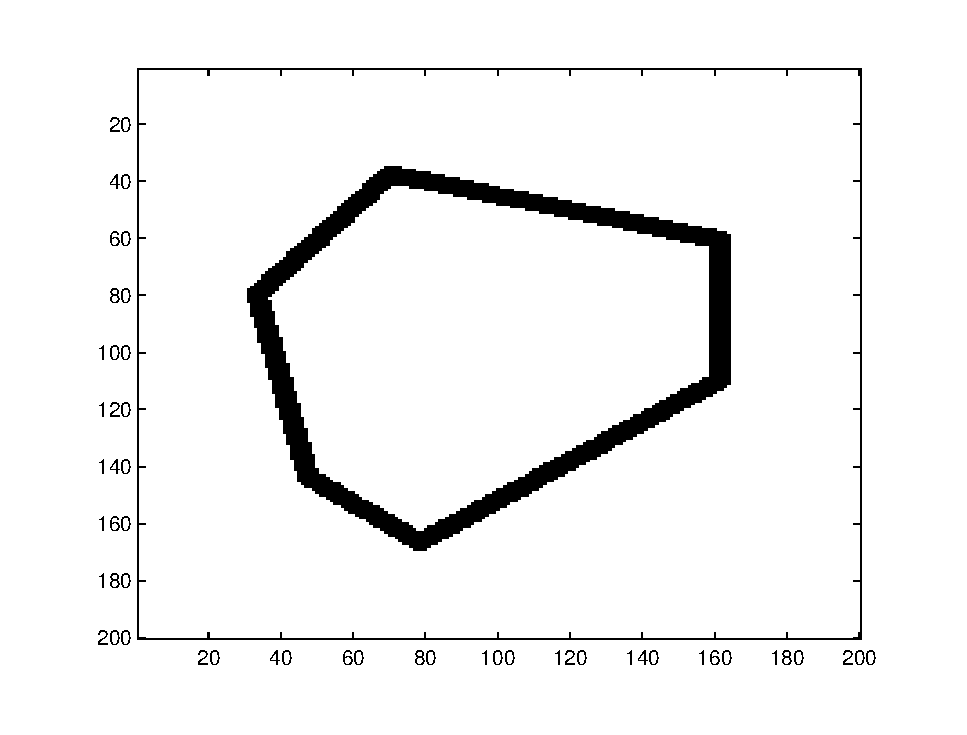
\includegraphics[width=0.49\textwidth]{pictures/membraneCellFull}\label{fig:membraneCellFull}}
\subfloat[Degraded synthetic Voronoi cell]{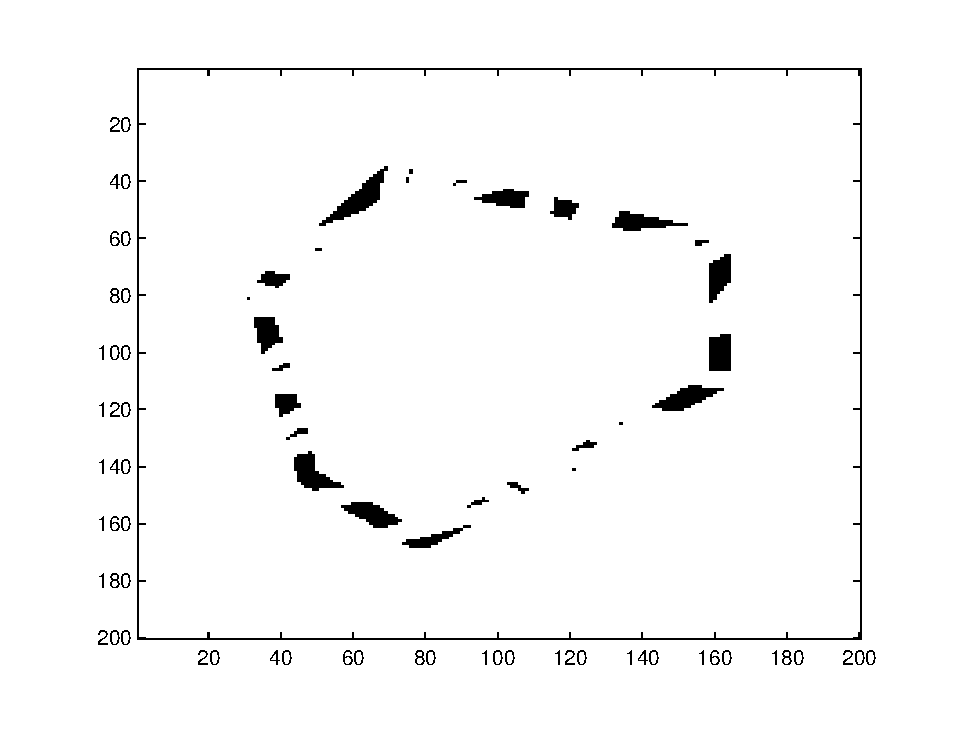
\includegraphics[width=0.49\textwidth]{pictures/membraneCellIncomplete}\label{fig:membraneCellIncomplete}}\\
\subfloat[Distance map computed from the synthetic Voronoi cell (figure~\ref{fig:membraneCellFull}). We clearly see a local maxima in the center of the cell.]{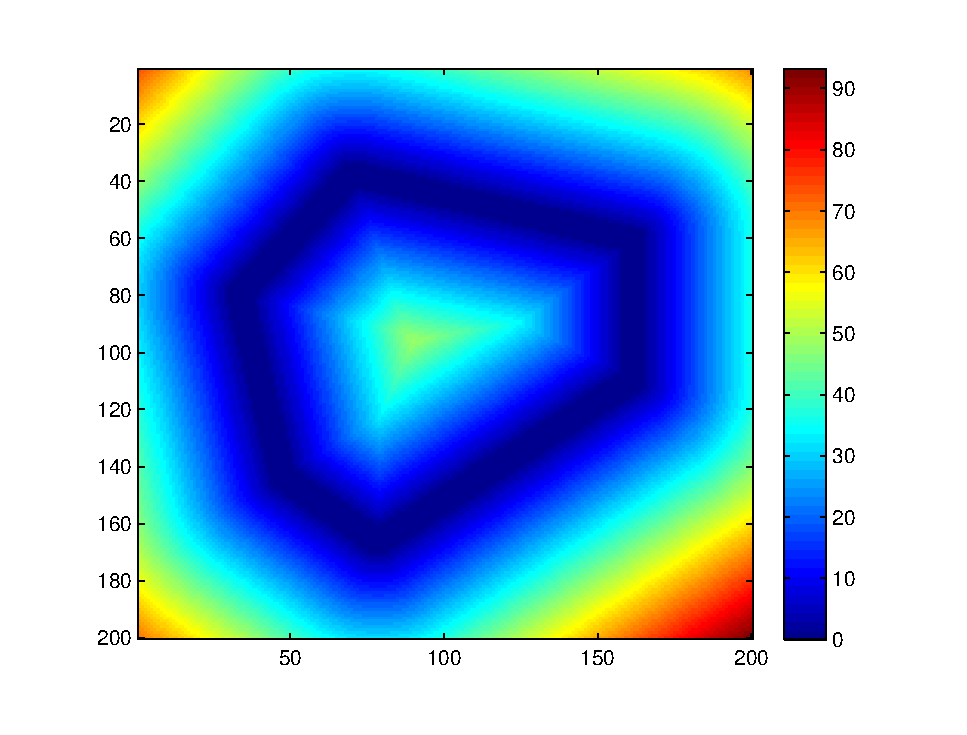
\includegraphics[width=0.49\textwidth]{pictures/membraneCellFullDistance}\label{fig:membraneCellFullDistance}}
\subfloat[Distance map computed from the degraded synthetic Voronoi cell (figure~\ref{fig:membraneCellIncomplete}). The local maxima is still in the center of the cell.]{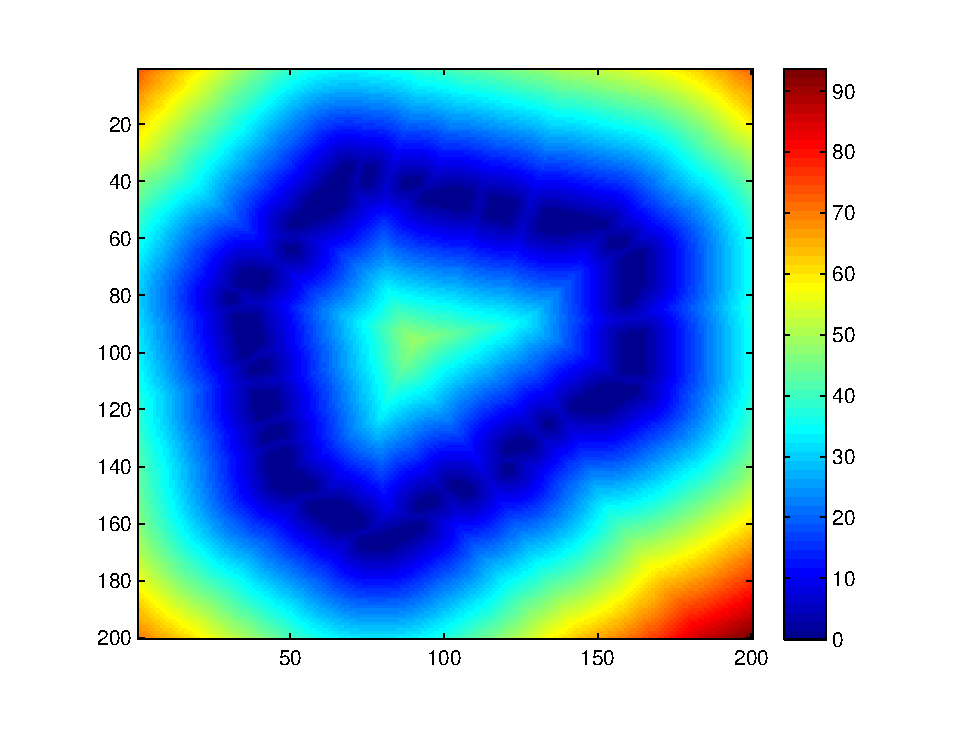
\includegraphics[width=0.49\textwidth]{pictures/membraneCellIncompleteDistance}\label{fig:membraneCellIncompleteDistance}}
\caption{Center of Voronoi cell stay unchanged under important degradation of the cell borders.}
  \label{fig:incompleteMembraneSynthetic}
\end{figure}

\paragraph*{}
We have seen that we can work on degraded membrane data to find an approximate position of cell nuclei.
We will now describe the innovative membrane reconstruction step that Kishore Mosaliganti developed and that we use in this algorithm.


This reconstruction is based on a diffusion filter pre-processing. The diffusion filter locates planar structures in the 3D data, and diffuses intensities along these plans.
We get a good first approximation of the membrane with this method, but many holes are still present.
In order to fill some of them, and reconnect the membrane, Kishore M.~{\etal} use a technique known as tensor voting.
This reconnect disconnected points, by finding privileged local directions.

The reconstruction of the membrane is illustrated figure~\TODO{reconstruction illustrations}.

This is the membrane information that we will use for finding the cell centres.





\subsubsection{Algorithm pipeline}

It is clear that for most image processing problems, a series of transformation is needed in order to be able to work with the data.
Inspired by the described articles, I designed an image processing pipeline adapted to our data.
I describe here the image processing pipeline for the new algorithm, and the improvements of the existing nuclei segmentation pipeline
\begin{description}
  \item[Denoising: ] We first process the membrane and the nuclei channel with a median filter. The median filter's structuring element is a disk of radius
  \TODO{radius of the median finally?}.
  We don't process directly the very low third dimension, as we may lose some relevant data,
  thus, the filter's structuring elements is two dimensional and applied to each "slice" (xy plan).
%
%
  \item[Images Resampling: ] As in \cite{li20073}, our images are anisotropic : they are very high resolution in xy, and very low resolution in z, as shown by the
  table~\ref{tab:DataSizes}, and the figure~\TODO{reference to the anisotropy figure in data analysis}.
  We don't need this much information in xy, as algorithms are computationally expensive, and we want to keep a reasonable processing time.
  But, we need a higher resolution in z.
  For that purpose, we resample our images, using a BSpline interpolation of order 5.
  This technique provides us with an isotropic dataset of spacing 0.4um, that can easily be
  processed by the other filters. The interpolation, in the z direction, partially reconstructs the membrane.
%
%
  \item[Nuclei binary mask: ] We threshold the nuclei image to keep a rough binary mask in which the nuclei are present.
  The thresholds are chosen after an analysis of the histogram of the nuclei images.
%  
  \TODO{image of the binary mask}
%
%  
  \item[Distance map creation: ] We then process the resampled and denoised membrane channel with Kishore's membrane reconstruction filter.
  The resultant membrane is thresholded to get a binary image from which we compute a distance map
  using the algorithm proposed by Maurer Jr {\etal}~\cite{maurer2003linear}.
  The threshold values are empirically determined.
%  
  \TODO{display distance map}
%
%
  \item[Local maxima extraction: ] Then, we dilate the distance map, This method is useful for local maxima extraction:
  it merges local maximas to keep the highest one, in a region defined by the structuring element's radius.
  After dilating the distance map according to , we locate local maximas with the flooding algorithm described in\cite{beare2005finding}.
  We only select local maximas that can possibly be located in the center of a cell, thus eliminating low values and high values corresponding respectively to holes in the membrane channel, and structures of the fish without cell.
%  
  \TODO{display dilated distance map}
%
%
\end{description}


\subsection{Evaluation}

It is important to note that often times, Biologists just want to count and localize objects in an image, without segmenting them.
That's why, in order to only evaluate the nuclei detection step, excluding the watershed segmentation, I created an evaluation framework providing necessary informations such as:
 out of nuclei detection (false positive), over detection of a nuclei (false positive), non detection of a nuclei (false negative) and correct detection of a nuclei.

I also created some tools for comparison of 3D datasets (based on {\gofigure}), and for simultaneous visualisation of point cloud and ray casted 3D dataset.

We will evaluate three algorithms in this section:
the algorithm that was used when I arrived in the Megason Lab (see section~\ref{sect:megasonExisting}),
the variant of the Laplacian of Gaussian presented in \cite{al2009improved} (see section~\ref{sect:farsight}),
and our proposed algorithm (see section~\ref{sect:proposal}).


\subsubsection{evaluation on synthetic data}

The generated synthetic data simulate the point-spread function of the microscope, on blobs, representing nuclei, and on Voronoi tessellations, representing membranes.
The data has a low resolution in z.
It is possible to have a variable noise level, and we will use these data to experience the robustness of the evaluated algorithms.

\begin{figure}[htb]
\begin{center}
\begin{tabular}{|c|c|c|c|c|}
\hline Noise level & Nuclei count & Correctly detected & Over-detected & Not-detected \\ 
%\hline x (space) & 1024 & 0.24 um & \\ 
\hline
\end{tabular} 
\end{center}
\caption{Evaluation of 3 algorithms on different synthetic datasets.}
\label{tab:DataSizes}
\end{figure}

\subsubsection{evaluation a segmented dataset}

We currently have one segmented dataset in the Megason Lab. The dataset is a part of an ear imaged 2 year ago. It is populated with a lot of noise. The region of interrest of the dataset (which has been manually segmented), contains \TODO{hox many cells in synthetic dataset ?} nuclei.
We ran the algorithms on the whole dataset, and masked the detection results with the region of interest.

\begin{figure}[htb]
\begin{center}
\begin{tabular}{|c|c|c|c|}
\hline Nuclei count & Correctly detected & Over-detected & Not-detected \\ 
%\hline x (space) & 1024 & 0.24 um & \\ 
%\hline y (space) & 1024 & 0.24 um \\ 
\hline
\end{tabular} 
\end{center}
\caption{Evaluation of 3 algorithms on a manually segmented dataset.}
\label{tab:DataSizes}
\end{figure}

\subsubsection{results}

\TODO{}
We found that THIS algorithm is more accurate, that THIS one is more robust, that THIS one is faster, that OURS is ...

\subsection{conclusion \& future}


We can improve the proposed algorithm, by automating the choice of the thresholds based on histograms.
We could also use non linear resampling methods, for improving the resolution among z.

We also implemented a Kdtree for grouping the local maximas, instead of using a dilation of the distance map,
such implementation would require a time evaluation, as the distribution of local maximas in space affects the effectiveness of the Kdtree requests.

We could combine the use of algorithms : the membrane based one in regions where nuclei are clumped, and the contour based ones (Kishore's or the improved Multiscale Laplacian of Gaussian) in region where nuclei are isolated.
The detection of such regions can be done by analysing the size of the connected components of the binarized nuclei image:
clumped nuclei correspond to large connected components.

\section*{Conclusion}


%A Context of the internship
%1- Biological Context / Goals
%2- Image Processing Challenges
%3- Data presentation
%4- The problem: you are going to address " ??? "
%
%B- Cell nuclei detection
%Intro
%1- State of the art
%2- What's wrong with existing method
%3- Your proposal
%4- Results
%    1- Synthetic data
%    2- Real data
%    3- Comparison of your method vs the other one. Validation? What is the benefit?
%5- Partial conclusion.
%    1- What is new?
%    2- Did you improve existing methods? in which way?
%        if not, why?
%    3- Future work.
%
%C- Membrane segmentation
%Intro
%1- State of the art
%2- What's wrong with existing method, if any?
%3- Your proposal (using a watershed starting from seeds)
%4- Results
%    1- Synthetic data
%    2- Real data
%    3- Comparison of your method vs the other one. Validation? What is the benefit?
%5- Partial conclusion.
%    1- What is new?
%    2- Did you improve existing methods? in which way?
%        if not, why?
%    3- Future work. 





%
%
%\subsection{Laplacian of Gaussian implementation}
%\label{sect:MLOG}
%\subsubsection{Strategy}
%
%\TODO{mettre dans les commentaires de farsight, improvements}
%
%The idea was to reimplement only the part of the algorithm of \cite{al2009improved} concerning the cell nuclei detection.
%The goal being to improve our initialization of the watershed algorithm. I was able to work with Raghav K. Padmanabhan, from the Roysam lab (who develops FTK),
%during the NA-MIC\footnote{The National Alliance for Medical Image Computing (NA-MIC) is a multi-institutional, interdisciplinary team of computer scientists,
%software engineers, and medical investigators who develop computational tools for the analysis and visualization of medical image data.} summer project week, in MIT.
%We tried to apply the FTK nuclei detection technique to 3D datasets, and to extract the Scale-constrained Laplacian of Gaussian implementation from the source code.
%
%A visual comparison of the binarization proceed by Kishore's algorithm and by the Farsight ToolKit led to the conclusion that Kishore's binarization
%was proceeding longer, but providing smoother results, which are important for the distance map step. That's the reason why, for the comparison of both algorithm,
%I reimplemented the Scale Constrained Laplacian of Gaussian and integrated it to Kishore's processing pipeline.
%
%
%\subsubsection{Implementation}
%After reading and understanding the article, I checked out the code from the Farsight Toolkit. The code has been developed two years ago and is not maintained any more.
%There was few documentation and comments, and the use of global variables made it hard to understand.
%I decided to start from scratch and reimplement the algorithm.
%
%The datasets are huge in the Megason Lab, and in order to process them, Kishore develops all his algorithms in \C++ with the Insight ToolKit (ITK) library.
%It was necessary that I develop the multi-scale Laplacian of Gaussian and create the whole evaluation framework with this language.
%
%
%\subsubsection{Testing}
%
%Prior to evaluating the algorithm, it was necessary to test it on some well known data.
%Indeed, The ITK implementation of the Multiscale Laplacian of Gaussian has a documentation and implementation problem:
% the code and the documentation are contradictory about the normalisation across scales.
%I tested the algorithm on a known function to verify its functioning.
%
%The test image was a 2D Gaussian of unit energy (integration across space equals one),
% and of different standard deviation. If the normalisation across scales is working,
%  the result of the Laplacian of Gaussian should be the same if computed across enough scales.
%\TODO{find the test for multiscale log on gaussian.}
%We proved the filter to be effectively working and detecting blobs of different scales without a loss in intensity as scale increases.
%\TODO{provide test for several scales}
%



%A "Plan of the internship"
%1 Goal (segment cells & membrane)
%2 Data presentation
%3 Where are we ? (membrane seg~0 cell seg needs lots of improvements)
%priority seeding imposed
%
%B Cell nuclei detection
% Intro
%bad seeding as of now, new ago, need for evaluation
%
%2 Biblio
%biblio on seeding evaluation
%
%3 Implementation
%implemantation … hard very hard (go through other's code forgotten already...)
%
%4 proposing
%new ago proposition new approach (based on membrane information)
%
%5 testing
%result of evaluation
%
%6 difficulties and future
%implementation big datasets 3D …
%future : merge results ? first : bad results everywhere : no more info for merging seedings...
%other ago based on wavelets? (as an opening)
%
%C Membrane segmentation
%  intro
%challenging need good cell detection...(but none present yet)
%1 biblio
%2 implementation (only 2D)
%3 result (only 2D)
%long very long but implementation can be greatly improved
%4 future
%not based on cell detection (start growing on the membrane)



%
%
%
%
%
%\section{Segmentation de la membrane cellulaire par ensembles de niveaux}
%
%Le but initial du PFE etait la segmentation de la membrane cellulaire. il s'agit d'une fine membrane séparant les multiples cellules. Elle s'étend sur tout le spécimen à analyser. Il s'agit donc d'un volume important et complexe.
%
%\subsection{Étude du problème}
%
%J'ai tout d'abord cherché à comprendre le problème posé : sur quelles données allaient se baser la détection, existe-t'il des solutions pour segmenter ce genre de données.
%
%\subsubsection{Les données}
%Les images sont acquises a travers un système optique. L'excitation par un laser entraine la fluorescence de certaines parties de la cellule, marquées par une molécule émettant de la lumière dans un spectre dépendant du marqueur utilisé.
%
%Le système a donc une réponse impulsionelle bien visible dans les données. Un point correspond grossièrement a une gaussienne étalée dans les trois dimensions de l'espace, et plus particulièrement selon l'axe perpendiculaire au plan de focalisation.
%
%Il existe aussi un bruit dû au dispositif électronique d'acquisition. De plus, la fluorescence n'étant pas répartie de manière homogène, il existe des "trous" et de la saturation dans les données.
%\TODO{inserer des images illustrant les problemes}
%
%
%J'ai choisi de me focaliser sur trois difficultés afin de trouver des solutions :
%\begin{description}
%  \item [problème du bruit] : quel filtrage appliquer aux images, afin de les débruiter.
%  \item [problème de l'absence de données] : comment introduire des à priori de forme de la membrane
%  pour palier à l'absence d'information ?
%  \item [problème de la non homogénéité des intensités]  : comment segmenter un objet
%  qui n'occupe pas les mêmes intensités selon sa position dans l'espace.
%\end{description}
%
%
%\subsection{Débruitage des données}
%Le bruit présent sur les images n'est pas gaussien. Il n'est pas répartis de la même manière dans toute l'image non plus. Je me suis donc focalisé sur des techniques de débruitage telles que le filtre médian, et plus généralement des filtres morphologiques.
%
%Le filtre médian donne de bons résultats, pour un temps de calcul inférieur aux filtres morphologiques (reconstruction par dilatation/erosion)
%
%\subsection{Segmentation de la membrane}
%
%\subsubsection{Utilisation de la théorie des ensembles de niveaux}
%
%L'outil choisi pour segmenter la paroi cellulaire, est base sur les ensembles de niveaux (levels-sets). Cette théorie consiste en l'évolution d'un front. Cette évolution est représentée par une fonction implicite qui évolue itérativement. Le front (bords de la zone segmentée) est souvent représenté par le niveau zéro de cette fonction implicite.
%Les Level sets, au travers de leur critère d'évolution, permettent d'avoir une grande flexibilité quand aux mesures a considerer lors de l'evolution du front. Cette évolution est représentée par un critère d'énergie, le problème de segmentation par level set est donc un problème d'optimisation.
%
%\subsection{des idees}
%
%
%
%
%
%
%idee de la mediane
%idee morphologie
%idee localisation
%\subsection{resultats}
%idee mediane
%idee morphologie
%idee localisation
%\subsection{travail futur}
%rapidite
%
%
%
%\section{Detection et localisation des cellules}
%
%Nous basons nos méthodes de segmentation sur une initialisation au centre des cellules. Nous avons donc besoin de détecter un maximum de cellules afin de trouver un point a l'intérieur de ces dernières. Des methodes ont ete proposees, cependant, chacune est adaptee a un type d'image particulier.
%Cels algorithmes de détection sont aussi souvent appelles algorithmes de "seeding" car ils permettent d'obtenir des points a partir desquels une segmentation peut etre initialisee, afin de delimiter les bordures des noyaux, ou les membranes cellulaires.
%
%\subsection{demarche}
%
%Nous avons developpe une methode combinant l'information provenant des noyaux et de la membrane des cellules. Cette methode doit etre evaluee, donc comparee a d'autres methodes existantes. Ce processus d'evaluation nous permettra aussi de trouver les points forts et les points faibles des algorithmes. Nous pourrons ainsi eventuellement utiliser des techniques de fusion d'information pour combiner les resultats de differents algorithmes.
%La creation d'un "framework" d'evaluation passe donc par plusieurs etapes : l'implementation des algorithmes existants, afin de les tester sur des images synthetiques puis reelles, la creation de criteres d'evaluation appropories, et l'observation des resultats. Nous avons aussi initié un travail afin de proposer une nouvelle methode de detection de cellules basee sur la decomposition en ondelettes.
%
%
%\subsection {description des algorithmes evalues}
%
%
%
%\subsubsection{chaine de traitement de l'image}
%
%partie commune
%Nous nous focalisons sur une classe d'algorithmes traitant l'information issue de l'image des noyaux cellulaires, apres une detection des zones d'interet (binarisation de l'image). Ces algorithmes fonctionnent aussi souvent avec une extraction de maxima locaux en dernier traitement.
%Nous choisissons d'utiliser la même binarisation, et la meme methode d'extraction de maximas locaux pour les deux algorithmes afin de focaliser l'etude sur la technique de detection des centres des noyaux.
%
%\subsubsection{description des algorithmes}
%\paragraph{le Laplacien de la Gaussienne ameliore}
%Nous avons decide d'implementer l'algorithme presente dans \cite{al2009improved}. La methode utilisee est celle du Laplacien de la Gaussienne (LoG). Une methode eprouveee qui s'est montree tres robuste dans d'autres applications telles la detection de points de reperes pour le recallage photographique.
%
%
%
%\paragraph{Kishore}
%
%\TODO{Ask Kishore more infos}
%
%
%\subsection {evaluation}
%%\begin{tabular}{|c|c|c|c|c|}
%%\hline  & Matching & UnMatching & Missed & Accuracy \\ 
%%\hline A1 & 10 & 3 & 1 & 71% \\ 
%%\hline A2 & 9 & 2 & 3 & 64% \\ 
%%\hline 
%%\end{tabular} 
%
%
%
%\subsection {conclusion}
%
%
%\subsection {proposition}
%
%
%
%\subsection {planning}
%
%
%\subsection{resultats}
%
%\subsection{proposition}
%
%
%
%


\chapter{State of the art}
\chapter{My Proposals}
\chapter{Results}


\chapter{Conclusion}
%
%
%
%\chapter{Conclusion du PFE}
%
%
%\section{Conclusion de la partie ingénierie}
%
%Durant ce PFE, j'ai travaillé sur des projets très variés.
%Ces projets étaient motivés par des objectifs scientifiques et nécessitaient chacun un haut niveau de technicité.
%
%J'ai eu l'occasion d'apprendre énormément,
%notamment dans le domaine des sciences informatiques,
%et du traitement de l'image.
%
%J'ai aussi découvert le milieu de la recherche, dont l'organisation est
%totalement différente de celle du milieu industriel.
%La hiérarchie, et les intérêts de chaque scientifique sont moins apparents que dans une entreprise et ce PFE a été riche en enseignements sur ce plan.
%Je suis parvenu à très bien m'intégrer dans l'équipe du Megason Lab en général,
%et à établir de bonnes relations de travail avec les divers scientifiques
%impliqués dans les projets sur lesquels j'ai travaillé.
%
%Cela m'a permis d'acquérir une base solide pour mener des recherches dans ce domaine.
%Après une importante phase d'apprentissage, je maitrise maintenant des librairies de renom
%(ITK, VTK,Qt), les systèmes unix, et la gestion de versions.
%
%J'ai pu aussi établir des contacts dans la communauté
%des traiteurs d'image par le biais de collaborations
%(Matthiew MacCormick), ou de d'"ateliers" (workshops) internationaux
%(participation à la NAMIC
%\footnote{La National Alliance for Medical Image Computing (NAMIC), est un réseau de professionnels de traitement d'images médicales. Ce réseau organise des conférences et des ateliers de travail ("workshop"), durant lesquels les scientifiques peuvent collaborer.}
%summer project week, au Massachusetts Institute of Technologies).
%
%
%\section{Projet professionnel}
%
%Ce PFE s'inscrit dans un projet professionnel construit durant ma scolarité à l'INSA de Lyon.
%Mon inscription à l'INSA de Lyon a été grandement motivée par l'ouverture de l'école à l'international. J'ai ainsi effectue mon stage ouvrier en Afrique du Sud. Profitant d'une première expérience professionnelle à l'international.
%
%Lors de ma seconde année a l'INSA de Lyon, j'ai choisi l'option SCiences et ANglais (SCAN).
%Cette filière regroupe les élèves ayant un niveau suffisant pour pouvoir suivre la formation généraliste en anglais.
%Elle s'accompagne d'une bourse pour un bref séjour linguistique dans une université étrangère.
%J'ai profité de ce financement pour aller au Trinity College en Irlande où
%j'ai pu avoir ma première expérience académique à l'étranger.
%
%J'ai ensuite choisi le département
%Génie Électrique qui permet de bénéficier d'un grand panel de compétences,
%notamment dans des domaines rattachés à l'électronique et l'informatique.
%
%
%Continuant l'expérience internationale, j'ai effectué mon stage industriel au
%Fraunhofer Institute, Center for Manufacturing Innovation, aux États Unis.
%J'ai été impliqué dans un projet de grande ampleur, financé par le département de la défense américain.
%Ce stage m'a énormément apporté en plus de l'expérience technique : il s'agissait d'une immersion dans la culture américaine, et j'ai eu une première expérience managériale en dirigeant une équipe d'ouvriers.
%C'est après ce stage que j'ai passé le test TOEIC validant un très bon niveau d'expression et de compréhension en anglais,
%avec un score de neuf cent quatre-vingt sur neuf cent quatre-vingt dix.
%
%
%Le PFE au Megason Lab possède des attraits indéniables :
%il s'agit d'un stage de recherche perfectionnant mes connaissances en traitement de l'image.
%Il s'agit aussi d'une expérience internationale dans une université renommée : Harvard Medical School.
%Ainsi, en plus de prendre plaisir à travailler en recherche, j'ouvre la porte à de nombreuses opportunités professionnelles.
%
%Comme je suis intéressé par les domaines techniques,
%je compte profiter de l'opportunité de poursuivre mes études pour obtenir un doctorat en mathématiques appliquées,
%au cours d'une thèse élaborée en collaboration avec le laboratoire CREATIS (INSA Lyon)
%et le laboratoire Megason (Harvard Medical School).
%Je passerai ainsi la moitié de mon temps en France, et l'autre moitié aux États Unis.
%En plus de pouvoir travailler sur un domaine passionnant,
%je pourrai ainsi bénéficier d'une équivalence avec un PhD (diplôme très reconnu à l'international). 
%
%Je compte ensuite mettre en valeur ma capacité a travailler dans un contexte international,
%dans des domaine à haute technicité pour trouver un emploi  dans le secteur privé.
%Je pourrai mettre en avant mes capacités en traitement du signal pour travailler dans le médical ou l'aéronautique.
%
%Mon ambition à long terme est de migrer vers des responsabilités managériales après avoir une très bonne maitrise de la technique.

\chapter*{Thanks}
\phantomsection
\addcontentsline{toc}{chapter}{Thanks}

I would like to thank, for their help and participation to my thesis, the following persons.

\begin{center}
Sean MEGASON\\
Kishore MOSALIGANTI\\
Arnaud GELAS\\
Olivier BERNARD\\
Rémy PROST\\
Matthiew MACCORMICK\\
Isabelle BLOCH\\
Nicolas RANNOU\\
Lydie SOUHAIT\\
Amelia GREEN\\
Nikolaus OBHOLZER\\
Ramil NOCHE\\
Raghav K. PADMANABHAN\\
Luis IBANEZ\\
\end{center}

And also the teams in Creatis LRMN, and in the Megason lab, for the great working ambiance I could find in these laboratories.

\appendix

%\section{The team}
%
%The Megason Lab's employee are post-doc researchers. Two domains of expertise are present : Biology and informatics.
%The biology team leads researches on the development of zebra fishes,
%and the computer team works on developing a program for visualization, segmentation, and tracking of cells adapted to microscopy data.
%
%{\small \begin{tabular*}{1.0\textwidth}{@{\extracolsep{\fill}} |  p{2.5cm} |  p{3.cm} | p{3.5cm} | c | }
%\hline Name & Status & Interest & Nationality \\ 
%\hline Sean Megason & Professor & Financing and managing the laboratory. & USA \\ 
%\hline Ramil Noche & Post-doctoral fellow & dynamics and function of gene regulatory networks. & Philipines \\ 
%\hline Fengzhu Xiong & Graduate student & cell differentiation mechanism to create neurons and skin cell. & Chine \\ 
%\hline Nikolaus Obholzer & Post-doctoral fellow  & Ear development and regeneration. &  Allemange \\ 
%\hline Paul Cowgill & Graduate student & Synthetic biology, noise and development. & USA \\ 
%\hline David Tulga & Graduate student & Cellular development. &  USA \\ 
%\hline Ian Swiburne & Post-doctoral fellow & Ear development. & USA \\ 
%\hline Andrea Tentner & Post-doctoral fellow  & Cell differentiation in spinal cord. & USA \\ 
%\hline Amelia Green & Post-doctoral fellow  & Variation and regulation in organ development. & Angleterre \\ 
%\hline Evan Schwab & Associate & Locations of genes responsible for mutations in the zebra fish ear using computational algorithm. & USA \\ 
%\hline Dante D'India & Technicien & Animal care. & USA \\ 
%\hline Arnaud Gelas & Research Engineer (senior) &  Developing {\gofigure}: Project management. &  France \\
%\hline Kishore Mosaliganti & Post-doctoral fellow  & Image processing algorithms, registration and segmentation. & India \\ 
%\hline Lydie Souhait & Research Engineer & Developing {\gofigure}: Responsible of the database (design, connexion, requests), and GUI & France \\
%\hline Nicolas Rannou & Research Engineer &  Developing {\gofigure}: Responsible of the visualization in {\gofigure} & France \\
%\hline Antonin Perrrot-Audet & Intern& Image processing : cells detection; developing {\gofigure} & France \\
%\hline 
%\end{tabular*} }

%\input{ingenierie/AnnexesIngenierie}

\bibliographystyle{plain}
\bibliography{AntoBib}

\end{document}
